\cotefile{154}
\scanpage{46}
% archive sheet number: 45

inverses des $D_i$ dans $\widetilde X$. (à ne pas confondre avec les revêtements des bords des $D_i$, quand on n'a pas choisi d'orientation de $D_i$)

\textcircled{$i$} On a une application

\[ \mathcal X \xrightarrow{\varphi} Y. \]

(application structurale) \inserted{quelles \deleted{\unsure{con}}ditions}

2) La restriction de $\varphi$ à \deleted{tt} face de $(\mathcal X,K)$ est un \deleted{\unsure{polygone}} \inserted{isomor\unsure{.}} \unsure{telle que}

% slanted
\margin{\unsure{Donc} \unsure{sauf les} \deleted{qu'elle construite} \deleted{en 2 \unsure{principes}} pour faces exceptionnelles, pour certaines arêtes, en un point !}

\deleted{1) L'ensemble $\Sigma$ \unsure{pte} à \unsure{$\varphi$ est fini} \unsure{$\mathrm{id}_{\mathcal X}$} $\mathcal X\smallsetminus K$}

Au voisinage de l'un \deleted{de tt point de $K\smallsetminus S(K)$,} \inserted{des bords de $K$,} $\varphi$ a la structure d'un ``folding'' d'arête.

3) Au voisinage de tt \deleted{pt} sommet de $K$, $\varphi$ a la structure d'un ``double folding'' relatif : $s$ et les deux branches de $K$ passant en $s$

4) \deleted{L'image \unsure{p} de tt sommet de $L$} \deleted{On a} \deleted{$\varphi^{-1}(\bigcup D_i)\cap K=\unsure{S}(L)\cap$} \deleted{($\Longrightarrow\varphi^{-1}(X_1)\cap K$} \quad $L=\varphi^{-1}(\underbrace{\bigcup D_i}_{X_1\deleted{\unsure{X_2}}})$

\margin{Considéré tel quel, il faudrait se placer en dehors des ``endroits'' autour des composantes de $K_0$}

Cor. \inserted{pour} \unsure{tt} pt de $S=K\cap L=(\varphi\mid K)^{-1}(X_1)$, \deleted{\illegible{1} est un} $\varphi(s)$ est un sommet, ssi \deleted{$s$ est un sommet de} \inserted{$s$ est ou bien un sommet de $K$, et est un sommet de $L$} \deleted{la carac. est le sommet critique de} --- i.e. est un \uline{point critique} de $K$. (l'un des pts est un coin t.t. que l'un des autres ordinaires de $K$).

\deleted{\unsure{j)} Soit.} j) Soit $F$ une face de $(\mathcal X,K)$. Considérons les \deleted{\unsure{éléments}} \inserted{pts} critiques de $K$ en $\partial F$, tels que la branche marquée en \deleted{\unsure{un sommet}} \inserted{$s$ (cf (d))} \deleted{\unsure{ou}} soit extérieure à $F$, et corrigeons le contour $\partial F$ par un petit renflement \deleted{de sorte que} \inserted{de façon} à ce que $s$ soit du côté privilégié de $s$.

\figure{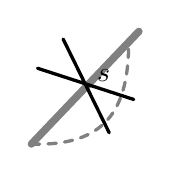
\begin{tikzpicture}[scale=.65,line cap=round]
\draw[line width=2.7pt,gray] (-1.1,-1.05)--(1,1.15);
\draw[gray,very thick,dashed] (-1.1,-1.05) .. controls (.35,-1.1) and (.8,-.38) .. (.8,.93);
\draw[very thick] (-.98,.43)--(.9,-.18) (-.48,1)--(.42,-.83);
\node at (.31,.29) {$s$};
\end{tikzpicture}}

% slanted
\margin{\uline{NB} \uline{(pour j)} Supposons pour \deleted{le voir} \unsure{seulement même} i.e. \unsure{$\exists$} un pt critique $s$ est sur le \unsure{vois} une face $F$ il \deleted{suffit} et s. que les \unsure{deux} \uline{branches de $L$} passant par $s$ se recoupent toutes en un autre point du bord de $F$ (dans le cas contraire, \deleted{les \unsure{autres deux}} qu'une au moins des deux branches sur le bord de $F$ sont trid\textsuperscript{les} et se rencontrent \unsure{cf} $F$ et $F'$ ci dessous}

\figure{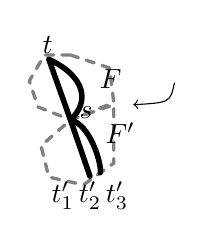
\begin{tikzpicture}[scale=.55,line join=round,line cap=round]
\draw[gray,very thick,dashed] (0,2)--(.9,1.7)--(1,.9)--(0,.5)--(-.75,.8)--(-.95,1.4)--(-.6,2)--cycle;
\draw[gray,very thick,dashed] (0,.5)--(1,.85)--(1,-.5)--(.3,-1)--(-.5,-.82)--(-.68,-.1)--cycle;
\draw[line width=2pt] (-.5,1.9)--(0,.5)--(.45,-.8) (-.5,1.9) .. controls (.35,1.5) and (.45,.92) .. (0,.5) .. controls (.45,.4) and (.72,-.5) .. (.69,-.72);
\node at (-.53,2.22){$t$};\node at (.36,.66){$s$};\node at (.93,1.45){$F$};\node at (1.15,.2){$F'$};\node at (.45,-1.25){$t'_1\,t'_2\,t'_3$};\draw[->] (2.4,1.35) .. controls (2.3,.9) .. (1.45,.85);
\end{tikzpicture}}

Soit \deleted{$\partial\unsure{F}$} $F'$ \deleted{\unsure{sa} la face \unsure{fermée}} \inserted{($F'\supset F$)} \deleted{\unsure{on trouve}} \inserted{on désigne} alors \deleted{\unsure{alors}} la partition relative correspondante : $\mathcal F$ est $\varphi(\partial' F)$, et \deleted{elle est} le système affine correspondant est canoniquement \deleted{isomorphe par} \inserted{isomorphe à} \deleted{$F',\unsure{\mathcal F}$} $(F',F'\cap L)$.

k) Appelons une arête exceptionnelle \uline{stable} ou instable (ou semi-stable) suivant que les deux \deleted{positions relatives} \inserted{faces} incidentes correspondantes : des pr. stables (resp. instables) (contiennent chacune resp. cont. \unsure{aucun}). Alors pour \deleted{\unsure{tout}} un sommet exceptionnel les bords privilégiés de la branche ord. de $K$ qui y passe est du côté de l'arête exc. instable (côté \unsure{fermé})

\scanpage{47}
% archive sheet number: 46

l) Loi de symétrie autour d'une arête exceptionnelle (comparer au \unsure{ré|n°} fin de e). et structure locale autour d'une composante exceptionnelle de $K$

\figure{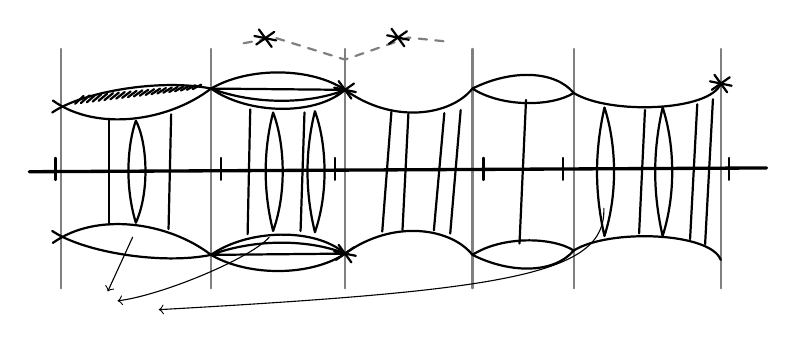
\begin{tikzpicture}[x=.83cm,y=.8cm,line cap=round,line join=round]
\foreach \x in {0,2.3,4.35,6.3,7.85,10.1}{\draw[gray,thick] (\x,-1.85)--(\x,1.95);}
\draw[very thick] (-.48,0)--(10.8,.06);
\foreach \x in {-.08,2.45,4.2,6.47,7.68,10.22}{\draw[thick] (\x,-.13)--(\x,.22);}
\foreach \s in {-1,1}{
\begin{scope}[yscale=\s]
\draw[thick] (-.13,.94) .. controls (.35,1.28) and (1.55,1.48) .. (2.3,1.32) .. controls (2.86,.91) and (3.89,.88) .. (4.35,1.3) .. controls (5.1,.74) and (5.98,.9) .. (6.3,1.32) .. controls (6.75,1.02) and (7.51,1.03) .. (7.85,1.25) .. controls (8.4,.9) and (9.94,.96) .. (10.1,1.4);
\draw[thick] (-.12,1.13) .. controls (.55,.63) and (1.65,.8) .. (2.3,1.32) .. controls (2.88,1.67) and (3.83,1.66) .. (4.35,1.3);
\draw[thick] (2.3,1.32)--(4.35,1.3) (2.3,1.32) .. controls (3,1.05) and (3.83,1.08) .. (4.35,1.3);
\draw[thick] (6.3,1.32) .. controls (6.9,1.63) and (7.56,1.61) .. (7.85,1.25);
\end{scope}}
\foreach \x/\h/\d in {.74/.84/0,1.65/.91/.04,2.86/.99/.04,3.67/.94/.06,4.92/.95/.14,5.23/.92/.09,5.71/.93/.16,5.96/.98/.16,7.02/1.14/.1,8.85/.98/.09,9.63/1.07/.11,9.86/1.15/.12}{\draw[thick] (\x,-\h)--(\x+\d,\h);}
\foreach \x/\h in {1.15/.81,3.25/.94,3.89/.96,8.32/1.02,9.21/1.02}{\draw[thick] (\x,-\h) .. controls (\x-.18,-.2) and (\x-.12,.46) .. (\x,\h) .. controls (\x+.17,.48) and (\x+.22,-.3) .. cycle;}
\foreach \x in {.22,.31,.40,.49,.58,.67,.76,.85,.94,1.03,1.12,1.21,1.30,1.39,1.48,1.57,1.66,1.75,1.84,1.93,2.02}{\draw[thick] (\x,{1.05+.13*\x})--(\x+.13,{1.18+.1*\x});}
\draw[gray,thick,dashed] (2.8,2.04)--(3.27,2.13)--(4.35,1.78)--(5.32,2.13)--(5.97,2.06);
\foreach \x/\y in {3.13/2.12,5.16/2.13,4.35/1.30,4.35/-1.30,10.10/1.40}{\foreach \a in {-55,-12,36}{\draw[thick] (\x,\y)++(\a:.17)--++(\a+180:.34);}}
\draw[thin,->] (1.1,-1.04)--(.72,-1.9);
\draw[thin,->] (3.19,-1.04) .. controls (2.9,-1.38) and (1.55,-1.96) .. (.87,-2.05);
\draw[thin,->] (8.31,-.58) .. controls (8.35,-1.64) and (6.8,-1.88) .. (1.5,-2.19);
\end{tikzpicture}}

figure \unsure{correcte|corrélée}, \deleted{\unsure{redéjà}} \unsure{voir} i) j) ---

\margin{\uline{NB} l'indice de chaque arête exceptionnelle stable est \deleted{\unsure{$=$}} $n-(\nu_{s_2}-1)-(\nu_{t}-1)$ \deleted{\unsure{$\nu_{s_2}$}} et les instables \deleted{\unsure{$=$}} $n-v$, où $v$ est la multiplicité du sommet --- où la figure ci-contre est concentrée ! On voit que l'indice des arêtes exceptionnelles résulte des autres données numériques}

m) Indexation des sections de $L$ sur les faces de $(\mathcal X,K)$ \deleted{à l'aide des} par $\widetilde I$, et passage d'une indexation à l'indexation de la face adjacente

n) Réconstitution de \deleted{$\unsure{\widetilde I}$} $\underline{\Sigma}$ (via $\widetilde I$ \unsure{---}) à l'aide de $K$, et des caractères numériques associés à $K$ (indices des \inserted{rd} sommets de $K$, \inserted{$2\nu(s)(-1)^{\unsure{\delta(s)}}$ où $\lambda(s)\in\mathbb N$,} $v(a)$ des arêtes \deleted{ordin\unsure{aires}} de $K$, \deleted{\unsure{et}} (distinguer le cas des arêtes ordinaires et des arêtes exceptionnelles.) Cf aussi

\uline{NB} Il y a aussi sûrement une loi de symétrie autour d'une arête ordinaire, pour ce qui est de la configuration induite par $L$ sur les 2 faces adjacentes, au voisinage de l'arête en question. Peut-être \deleted{\unsure{un}} en tous cas : Considérons la carte $(\mathcal X,K\cup L)$, et ``le voisinage tubulaire stand. et ``Thurénien'' d'arêtes'' de \deleted{$K$ des arêtes} \inserted{son sous-graphe $K$ de} $K\cup L$ dans cette carte. \deleted{considérons} Alors, pour tte $\unsure{a|te}$ arête $a$ de $K$, \unsure{posant}

\figure{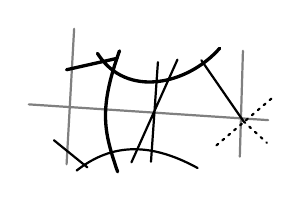
\begin{tikzpicture}[scale=.8,line cap=round]
\draw[gray,thick] (0,-.8)--(.12,1.35) (-.6,.15)--(3.2,-.1) (2.75,-.68)--(2.8,1);
\draw[very thick] (0,.7)--(.8,.88) (.49,.96) .. controls (.95,.23) and (1.93,.47) .. (2.43,1.04);
\draw[very thick] (.84,1) .. controls (.5,.05) and (.6,-.3) .. (.81,-.92);
\draw[thick] (1.45,.82)--(1.34,-.76) (1.76,.86)--(1.03,-.77) (2.14,.85)--(2.81,-.12);
\draw[thick] (-.2,-.42)--(.33,-.85) (.16,-.9) .. controls (.65,-.52) and (1.24,-.4) .. (2.08,-.86);
\draw[dotted,thick] (2.38,-.5)--(3.25,.24) (2.81,-.12)--(3.18,-.46);
\end{tikzpicture}}

$T_a\overset{\mathrm{déf}}{=}(F'\cup F'')\cap T$, où $F',F''$ sont les deux faces de $(\mathcal X,K)$ incidentes à $a$, on a une involution \deleted{\unsure{$\varphi$}} $\sigma_a$ de $a$, ayant en commun un des pts fixes, et respectant la structure cellulaire induite par $(\mathcal X,K\cup L)$. De plus, \deleted{si $a$ et $b$} sont incidentes au m sommet $s$, alors $\sigma_a\mid T_a\cap T_b$ et $\sigma_b\mid T_a\cap T_b$ commutent dans un sens évident

\scanpage{48}
% archive sheet number: 47

\unsure{7|2}.2.1984

\uline{Structure de $K$} On rajoute des sommets d'ordre 2, soit $S_K$ l'ens des sommets. On désigne par $K$ le graphe top. avec ses nouveaux sommets. (les anciens sont ceux de l'\deleted{$K$}ordre 4). On a

\[ S_K=\underbrace{S'_K}_{\substack{\text{sommets}\\\text{rouges}}}\amalg
\underbrace{S''_K}_{\substack{\text{sommets}\\\text{\deleted{rouges}\inserted{noirs}}}} \]

\margin{\uline{NB} \deleted{$I$ \unsure{et} $S_K$ \unsure{que} $S''$} \inserted{$S'_K$ contient des} sommets d'ordre 2, pas néc. des sommets d'ordre 4 $S''_K$ contient des sommets d'ordre 2 pas néc. d'ordre 4}

avec :

a) Pour tte \deleted{\illegible{1}} face $F$, $S'_K\cap F$ et $S''_K\cap F\unsure{_2}$ st des subdivisions de $\partial F$ duales l'une de l'autre, d'ordre $2n$

\deleted{\unsure{b)}} \uline{NB} --- Deux sommets consécutifs sur $\partial F$ ne sont pas d'ordre 4, et \deleted{plus} précisément, \deleted{\unsure{entre deux}} sur un arc de $\partial F$ joignant deux sommets d'ordre 4, il y a toujours au moins un sommet rouge d'ordre 2, (et même deux si $\Sigma$ n'est pas \deleted{d'ordre} du type $\mathrm{II}_p$ et on est sur une arête exceptionnelle) et au moins un sommet noir (si on n'est \unsure{B}| par tous les cas qu'on vient de dire\ldots)

b) \deleted{Intro} On a une section du fais des visées pour le déploiement $K'$ de $K$. Ainsi, chaque arête $a$ d'une face \inserted{$F$} est munie d'un signe $\varepsilon_F(a)$, qui est \deleted{\unsure{$\pm$}}$+1$ si la visée est du côté de $F$, $-1$ sinon. On a les règles

\[
\left\{\begin{aligned}
\varepsilon_{F'}(\unsure{a'})&=-\varepsilon_F(a) &&\text{si $F,F'$ sont les deux faces incidentes à $a$}\\
\varepsilon_F(\unsure{a})&=\varepsilon_{\unsure{F}}(\unsure{b}) &&\text{si $a$ et $b$ sont adjacentes sur $F$, le sommet commun étant d'ordre 2}\\
\varepsilon_{a_1}(F_1)&=\varepsilon_{a_2}(F_2) &&\text{si $F_1$ et $F_2$ sont adjacentes le long d'une}\\[-2pt]
&&&\text{arête mitoyenne $b$, d'extrémité $s$, d'ordre 4}\\
&&&\text{et quand $a_1$ et $a_2$ sont incidentes à $F_1$ et $F_2$}\\
&&&\text{respectivement, $\ne b$, et incidentes à $s$.}
\end{aligned}\right.
\]

\figure{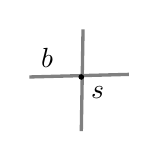
\begin{tikzpicture}[scale=.55]\draw[gray,very thick] (-1.2,0)--(1.1,.06) (0,-1.25)--(.04,1.1);\fill (0,0) circle (.065);\node[above] at (-.79,0){$b$};\node[below right] at (0,0){$s$};\end{tikzpicture}}

Il résulte du fait que \deleted{\unsure{l tes}} les faces sont de même ordre $4n$, que pour \deleted{deux arêt} toute arête $a$, si $F,F'$ sont les deux faces incidentes, on a une \unsure{som|sorte} de \uline{symétrie autour de $a$}

\margin{\uline{NB} on a $\sigma_a^F\sigma_a^{F'}=\mathrm{id}$}

\[ \sigma_a^F\text{ ou }\sigma_a:\quad \deleted{\unsure{F}}\operatorname{Pol}(F)\xrightarrow{\sim}\operatorname{Pol}(F') \]

caractérisé par la condition de laisser \deleted{invariants} \inserted{fixes} les deux extrémités de $a$. Il laisse alors \deleted{invariants} \inserted{fixes} \deleted{toutes} tous les sommets et arêtes qui sont sur la ``grande arête'' $\widehat a$ contenant $a$ (bordée par les sommets d'ordre 4 les plus proches) (mais \deleted{pas les \unsure{prochai}} \inserted{les prochains sommets sur $\partial F$} (de part et d'autre de $\widehat a$ sont non fixés par $\sigma_a$). L'application $\sigma_a$ transforme sommets rouges (resp. noirs) en sommets noirs

% slanted
\margin{\uline{NB} $\sigma_a^F=\sigma_{a'}^F$ si $a$, $a'$ sont sur la même \uline{grande arête}}

\scanpage{49}
% archive sheet number: 48

2.1.84

\deleted{On place sur $K$ des nouveaux sommets (d'ordre 2), de la façon suivante ; \deleted{Pour On \unsure{fixe} par faces (soit $F$) de \unsure{quelles}, on prend les sommets} arête par arête fermée.}

\deleted{a) On rajoute les pts de $K\cap L$ sur $\partial F$}

\deleted{b) Pour toute arête du nouveau complexe topologique $(\partial F,S\cap\partial F\cup(\partial F\cap L)$, \deleted{\unsure{on en}} distinguer}

\figure{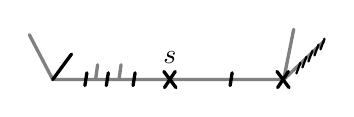
\begin{tikzpicture}[scale=.85,line cap=round]
\draw[gray,very thick] (-.35,.67)--(0,0)--(3.45,0)--(3.6,.75) (3.45,0)--(4.05,.57);
\draw[very thick] (0,0)--(.28,.38);
\foreach \x in {.48,.80,1.2,2.65}{\draw[very thick] (\x,-.09)--(\x+.03,.1);}
\foreach \x in {.64,.99}{\draw[gray,very thick] (\x,0)--(\x+.03,.22);}
\foreach \x in {1.75,3.44}{\draw[very thick] (\x-.08,-.12)--(\x+.08,.12) (\x-.09,.12)--(\x+.09,-.12);}
\node[above] at (1.75,.1){$s$};
\foreach \x in {0,.09,.18,.27,.36}{\draw[thick] (3.64+\x,.09+\x)--(3.7+\x,.25+\x);}
\end{tikzpicture}}

\figure{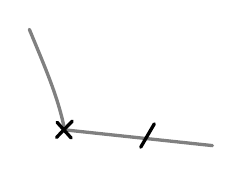
\begin{tikzpicture}[scale=.69,line cap=round]\draw[gray,very thick] (-.65,1.85) .. controls (-.34,1.1) and (-.12,.6) .. (0,0)--(2.72,-.29);\draw[very thick] (-.15,-.14)--(.14,.16) (-.14,.14)--(.12,-.15) (1.4,-.32)--(1.65,.11);\end{tikzpicture}}

\deleted{a) On rajoute les pts de $\bar a\cap L$ --- soit $\underline a'=(a,a\cap S(K)\cup a\cap L)$ le graphe-segment \inserted{top} obtenu, soit $\alpha$ une arête de ce graphe.}

\deleted{(\uline{NB} \deleted{\unsure{Il}} Il y a au moins un \deleted{a) Si une des ext} élément de $a\cap L$ (\deleted{arête} ``sommet rouge'') sur $a$ distinct des extrémités, donc chaque arête $\alpha$ de $\underline a'$ \deleted{\unsure{cont}} a au moins une extrémité rouge, i.e. qui n'est pas une \deleted{sommet} \inserted{extrémité} de $\underline a$, et il y en a exactement deux qui n'en ont qu'une de rouge (l'autre étant verte)).}

\deleted{a) Sur ces dernières, on ne rajoute pas d'autre sommet \inserted{(sauf si l'extr\unsure{émité} en $a$ est un sommet de la} \deleted{\unsure{b)} Sur toute} Pour les autres arêtes, on \deleted{dis}rajoute des sommets (oranges) de la façon suivante}

\deleted{b) Si \deleted{les} les \inserted{deux} extrémités sont non critiques i.e. ne sont pas des sommets de $L$, on rajoute juste un sommet (le milieu)}

\deleted{c) \deleted{Si un} Pour les deux autres arêtes (cas d'une arête $\underline a$ ordinaire), de part et d'autre du pt critique \deleted{\unsure{$t$}} $s$, si $\nu(s)$ est son ordre, on dispose $\frac{\nu(s)}2$ pts rouges (si}

\scanpage{50}
% archive sheet number: 49

J'aimerais comprendre la relation entre les $\sigma_a^F$, et les signes $\varepsilon_F(a)$.

Mais il faut encore introduire une autre structure

c) L'ensemble $C_K\subset S_K$ des ``pts critiques'' avec la condition que \inserted{ils sont d'ordre 2, et que} sur chaque \deleted{\unsure{ar}} grande arête, il y a \deleted{\unsure{au plus}} \inserted{exactement} un \deleted{tel} élément de $C_{\unsure{K|F}}$ \deleted{(quand il n'y en a pas, l'arête est dite \uline{exceptionnelle}).} De plus, chaque p\unsure{ts|t} critique $s$ est muni d'un poids $\nu(s)\geq\deleted{\unsure{2}}1$, \inserted{qui est pair ou impair, suivant que $s$ est noir, ou \deleted{orange}} (le poids d'un élément de $S_K$ est par définition $\nu(s)$ si \unsure{critique}, 1 si $s$ non critique \deleted{\unsure{du pt}} et de $S'_K$, 0 s'il est non critique \deleted{et} est de $S''_K$)

\margin{définir les ``arcs critiques'' ou ``arcs de transition'' sur les arêtes, d'amplitude totale $2\nu(s)$ (il contient $\nu(s)$ sommets \deleted{de $S'_K$} rouges, et ses extrémités sont \unsure{rouges|oranges})}

% slanted
\margin{\uline{NB} Les arcs de transition (fermés) sont mutuellement disjoints}

% slanted
\margin{Les pts critiques sont les centres des arcs critiques, et déterminent les paliers (comme la moitié de l'amplitude correspondante du cas entier) --- donc il \unsure{revient précisément} au même de se donner ces arcs critiques.}

% slanted
\margin{les sommets d'ordre 4 sont exactement \deleted{\unsure{ceux qui}} les milieux des arcs \deleted{\unsure{complémentaires}} \inserted{compris} \deleted{\unsure{par}} entre les arcs \deleted{de transition} \inserted{critiques}}

En termes des sommets critiques, on a ceci :

1) Soit $s$ un sommet critique, incident à la face $F$. Soit $s'$ son antipodique dans $\partial F$. \deleted{Alors si $s'$ est non critique, on doit le signe $\varepsilon_a$} \inserted{Pour qu'on ait $\varepsilon_F(a)=+1$, il f et s.} que le sommet $s'$ antipodique \deleted{\unsure{$t$}} de $s$ \inserted{pour $F$} soit égalmt critique (il a alors le même indice)

% slanted
\margin{relation entre $C_K$ et les signes $\varepsilon_F(a)$}

2) Sur toute face $F$, il y a au moins 3 pts critiques sur $\partial F$ (et même au moins 4, \deleted{\unsure{3)} si tous les pts} il y a au moins un pt critique \inserted{$s$} de signe $+1$. \deleted{\unsure{aura faites}} \inserted{Dans ce cas,} sur chacune

\scanpage{51}
% archive sheet number: 50

2.1.84.

\deleted{On place sur \deleted{\unsure{chque}} $K$ deux ensembles de pts, $S'_K$ $S''_K$\deleted{\unsure{$''$}} \deleted{\unsure{de}}, de telle façon que}

\inserted{$S'_K$ : sommets rouges \quad $S''_K$ : sommets oranges}

\deleted{\deleted{\unsure{b)}} $\forall\,F$ face de $K$, $\partial F\cap S'$ est un polygone top. d'ordre $2n$, et sur chaque arête \inserted{$\alpha$} \deleted{il y} de celui ci il y a un pt de $S''$ et un seul, qui est son milieu si $\alpha$ est contenu}

\deleted{a) $\forall\,S'_K$ \unsure{de} \unsure{tt} \unsure{pt} tous les sommets} \deleted{a) $S'_K\supset S(K)$, $S'_K\supset\unsure{S_2}K\cap L\smallsetminus K\cap S(L)$}

\deleted{a) $S'_K\cap L=K\cap L\smallsetminus(\text{ensemble des pts critiques de $K$ qui sont d'ordre pair})$}

\deleted{b) $S'_K\cap S(K)=S(K)\cap L$}

\deleted{b) \deleted{\unsure{Tout}} Pour toute arête (anc.) $a$ de $K$, on a $a\cap S'_K\ne\varnothing$.} \inserted{\deleted{dans \deleted{une} arête de $K$, et l'unique sommet de $K$ sur $\alpha$ dans le cas inverse.}}

\figure{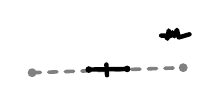
\begin{tikzpicture}[x=0.008cm,y=-0.008cm,line cap=round,line join=round]
\draw[gray,line width=1.3pt,dashed] (0,45)--(240,37);
\draw[line width=1.6pt] (90,40)--(151,39);
\draw[line width=1.6pt] (118,32)--(119,49);
\fill[gray] (0,45) circle [radius=1.6pt];
\fill[gray] (240,37) circle [radius=1.6pt];
\fill[black] (90,40) circle [radius=1.2pt];
\fill[black] (151,39) circle [radius=1.2pt];
\draw[line width=1.6pt] (205,-14)--(212,-14)--(215,-9)--(217,-22)--(220,-13)--(223,-19)--(226,-13)--(230,-23)--(233,-11)--(250,-16);
\end{tikzpicture}}

\figure{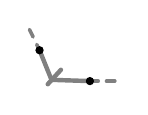
\begin{tikzpicture}[x=0.008cm,y=-0.008cm,line cap=round,line join=round]
\draw[gray,line width=1.3pt,dashed] (0,0)--(16,33);
\draw[gray,line width=1.6pt] (16,33)--(35,80)--(96,82);
\draw[gray,line width=1.6pt] (29,87)--(50,64);
\draw[gray,line width=1.3pt,dashed] (96,82)--(140,82);
\fill[black] (16,33) circle [radius=1.5pt];
\fill[black] (96,82) circle [radius=1.5pt];
\end{tikzpicture}}

\deleted{\unsure{Ex} \uline{NB} a) et b) impliquent que $S'_K\cap S(K)=S(K)\cap L$ i.e. un sommet de $K$ est dans $S'_K$ sss il est dans \unsure{la|L}}

\deleted{c) \deleted{$S'_K\smallsetminus S'_K\cap L$ est réunion de segments, un pour chaque} P\unsure{r} un \unsure{tt} pt critique $s$ de $K$, sur l'arête \deleted{arête} \inserted{de} ord \deleted{\unsure{notée $a$}} \inserted{$K$} \deleted{$a$ qui} désignant par $t',t''$ les pts les plus proches de $s$, sur l'arête $a$ de $K$ contenant $s$, parmi les pts de $(a\cap L)\cap\partial a$ \deleted{on dispose sur le segment $[t',t'']$} \inserted{l'intersection $[t',t'']\cap S'_K$ est de cardinal égal à} $\nu(s)$, \deleted{et il y a la}}

\figure{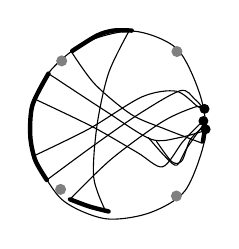
\begin{tikzpicture}[x=0.007cm,y=-0.007cm,line cap=round,line join=round]
\draw[thin] plot[smooth cycle] coordinates {(42,78) (108,23) (196,2) (275,34) (317,118) (326,195) (290,291) (224,332) (144,342) (66,307) (18,229) (9,149)};
\draw[line width=1.6pt] plot[smooth] coordinates {(85,38) (130,10) (160,1) (193,1)};
\draw[line width=1.6pt] plot[smooth] coordinates {(42,79) (13,136) (9,192) (18,236) (39,272)};
\draw[line width=1.6pt] plot[smooth] coordinates {(81,307) (116,320) (151,329)};
\draw[line width=1.6pt] plot[smooth] coordinates {(324,164) (326,177) (322,202)};
\fill[gray] (66,56) circle [radius=2pt];
\fill[gray] (275,39) circle [radius=2pt];
\fill[gray] (64,289) circle [radius=2pt];
\fill[gray] (274,301) circle [radius=2pt];
\draw[thin] plot[smooth] coordinates {(188,2) (151,78) (130,173) (124,267) (145,327)};
\draw[thin] plot[smooth] coordinates {(84,40) (126,98) (192,153) (252,179) (320,205)};
\draw[thin] plot[smooth] coordinates {(42,79) (144,146) (228,198) (280,195) (327,182)};
\draw[thin] plot[smooth] coordinates {(21,127) (123,176) (203,222) (249,248) (286,202) (322,165)};
\draw[thin] plot[smooth] coordinates {(16,228) (116,179) (212,121) (274,111) (313,139) (327,143)};
\draw[thin] plot[smooth] coordinates {(39,272) (119,213) (205,153) (281,110) (307,125) (324,143)};
\draw[thin] plot[smooth] coordinates {(81,307) (156,234) (249,166) (310,139) (325,143)};
\draw[thin] plot[smooth] coordinates {(223,195) (255,231) (275,245) (293,214) (322,173)};
\draw[thin] plot[smooth] coordinates {(238,202) (266,239) (284,237) (299,199) (321,177)};
\fill[black] (325,143) circle [radius=1.8pt];
\fill[black] (323,165) circle [radius=1.8pt];
\fill[black] (327,180) circle [radius=1.8pt];
\end{tikzpicture}}

\figure{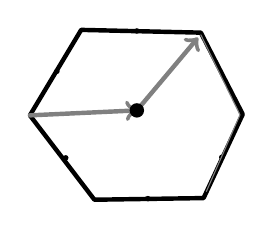
\begin{tikzpicture}[x=0.007cm,y=-0.007cm,line cap=round,line join=round]
\draw[line width=1.6pt] (0,155)--(93,0)--(310,5)--(386,153)--(315,305)--(117,308)--cycle;
\fill[black] (49,75) circle [radius=1pt];
\fill[black] (194,2) circle [radius=1pt];
\fill[black] (348,231) circle [radius=1pt];
\fill[black] (214,306) circle [radius=1pt];
\fill[black] (65,232) circle [radius=1pt];
\draw[gray,line width=1.6pt,->] (0,155)--(194,146);
\draw[gray,line width=1.6pt,->] (194,146)--(305,14);
\fill[black] (194,146) circle [radius=2.6pt];
\draw[gray,thin] (310,9)--(381,154)--(320,293);
\end{tikzpicture}}

\figure{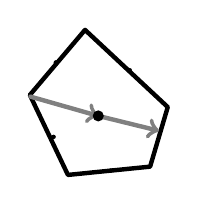
\begin{tikzpicture}[x=0.007cm,y=-0.007cm,line cap=round,line join=round]
\draw[line width=1.6pt] (0,118)--(100,0)--(250,140)--(218,248)--(69,263)--cycle;
\fill[black] (47,59) circle [radius=.8pt];
\fill[black] (181,73) circle [radius=.8pt];
\fill[black] (147,255) circle [radius=.8pt];
\fill[black] (43,194) circle [radius=.8pt];
\draw[gray,line width=1.6pt,->] (1,121)--(124,156);
\draw[gray,line width=1.6pt,->] (124,156)--(234,183);
\fill[black] (124,156) circle [radius=2pt];
\end{tikzpicture}}

\figure{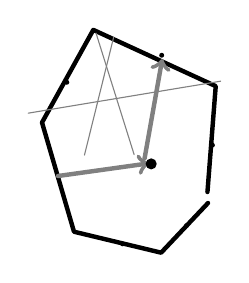
\begin{tikzpicture}[x=0.007cm,y=-0.007cm,line cap=round,line join=round]
\draw[line width=1.6pt] (300,304)--(315,112)--(93,10)--(0,178)--(58,376)--(216,414)--(301,324);
\fill[black] (45,105) circle [radius=.9pt];
\fill[black] (217,56) circle [radius=.9pt];
\fill[black] (309,219) circle [radius=.9pt];
\fill[black] (262,365) circle [radius=.9pt];
\fill[black] (146,398) circle [radius=.9pt];
\fill[black] (30,276) circle [radius=.9pt];
\draw[gray,line width=1.6pt,->] (29,275)--(194,252);
\draw[gray,line width=1.6pt,->] (186,243)--(218,63);
\fill[black] (198,253) circle [radius=2pt];
\draw[gray,thin] (-25,161)--(324,103);
\draw[gray,thin] (130,23)--(77,237);
\draw[gray,thin] (98,16)--(167,236);
\end{tikzpicture}}

\figure{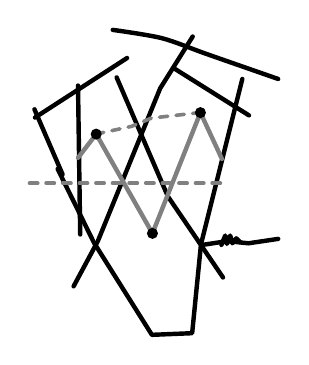
\begin{tikzpicture}[x=0.007cm,y=-0.007cm,line cap=round,line join=round]
\draw[line width=1.6pt] (9,182)--(60,300);
\draw[line width=1.6pt] (51,290)--(117,424)--(222,591)--(295,588)--(311,427)--(386,127);
\draw[line width=1.6pt] (80,503)--(124,421)--(237,144)--(296,50);
\draw[line width=1.6pt] (158,124)--(251,340)--(351,487);
\draw[line width=1.6pt] (88,139)--(92,409);
\draw[line width=1.6pt] (10,197)--(177,89);
\draw[line width=1.6pt] plot[smooth] coordinates {(151,38) (240,53) (322,82) (451,127)};
\draw[line width=1.6pt] (261,107)--(398,193);
\draw[line width=1.6pt] (313,428)--(359,421)--(397,425)--(451,417);
\draw[gray,line width=1.6pt] (88,270)--(121,227)--(223,407)--(310,188)--(349,272);
\draw[gray,line width=1.3pt,dashed] (120,227)--(185,213)--(221,198)--(309,188);
\draw[gray,line width=1.3pt,dashed] (0,316)--(355,316);
\fill[black] (121,227) circle [radius=2pt];
\fill[black] (223,407) circle [radius=2pt];
\fill[black] (310,188) circle [radius=2pt];
\draw[line width=1.6pt] (348,428)--(355,411)--(358,426)--(364,411)--(368,425)--(375,416)--(382,423);
\end{tikzpicture}}

\figure{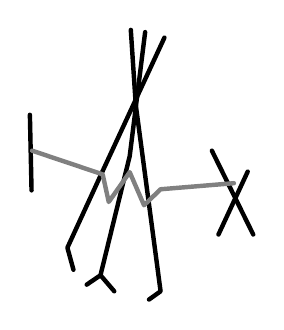
\begin{tikzpicture}[x=0.007cm,y=-0.007cm,line cap=round,line join=round]
\draw[line width=1.6pt] (0,140)--(3,277);
\draw[line width=1.6pt] (79,421)--(68,381)--(131,244)--(244,0);
\draw[line width=1.6pt] (103,448)--(128,431)--(181,215)--(209,-10);
\draw[line width=1.6pt] (129,432)--(153,460);
\draw[line width=1.6pt] (183,-14)--(192,122)--(237,460)--(216,475);
\draw[line width=1.6pt] (330,205)--(405,357);
\draw[line width=1.6pt] (342,357)--(395,243);
\draw[gray,line width=1.6pt] (4,205)--(132,248)--(143,298)--(181,244)--(207,304)--(237,275)--(370,264);
\end{tikzpicture}}

\scanpage{52}
% archive sheet number: 51

\deleted{\illegible{1}} des deux arcs \inserted{ouverts} déterminés par $s,t$ sur $\partial F$, il y a au moins un pt critique

d) \uline{Relation entre} sommets critiques \deleted{\unsure{de}} sur $F$ et sur $F'=\sigma_a(F)$ $a$ une \uline{grande arête} sur $\partial F$. \unsure{UPS|DPS} que $\varepsilon_F(a)=+1$ (quitte à intervertir les rôles de $F$ et $F'$). On a donc ceci : Soit \deleted{$s$ le pt critique sur $a$,} \inserted{$t$ l'antipodique de $s$, qui est critique,} $u,v$ les deux pts critiques les plus voisins de \deleted{$\partial F$} \unsure{$t|s$}, de part et d'autre de $s$, \deleted{\unsure{$s$}} $\beta=\widehat{u\unsure{t}v}$ l'arc correspondant \inserted{de $\partial F$,} d'extrémités $u,v$ contenant $s$. Considérons \deleted{$\beta=$} l'autre arc d'extrémités $u$ et $v$, soit $\alpha$. \deleted{Soient} (NB, on a $u,v$ sur \deleted{deux} arcs \inserted{ouverts} distincts déterminés par $s,t$ sur $\partial F$, \deleted{donc} et $u\ne v$, donc $s\in\deleted{\beta}\alpha$, de façon précise $\alpha=\widehat{usv}$). \deleted{Soient} \inserted{$s'=s$,} $t',u',v'$ \deleted{leurs} transformés de $s,t,u,v$ par $\sigma_a$.

\figure{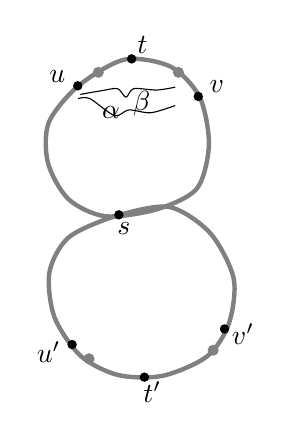
\begin{tikzpicture}[x=0.009cm,y=-0.009cm,line cap=round,line join=round]
\draw[gray,line width=1.6pt] plot[smooth cycle] coordinates {(55,47) (120,10) (185,20) (226,63) (239,130) (222,192) (166,221) (93,231) (41,207) (12,156) (13,99)};
\draw[gray,line width=1.6pt] plot[smooth cycle] coordinates {(107,231) (183,218) (241,255) (274,319) (267,383) (236,429) (174,456) (111,455) (58,428) (21,373) (14,310) (41,261)};
\fill[black] (54,47) circle [radius=1.7pt];
\fill[black] (130,9) circle [radius=1.7pt];
\fill[black] (224,62) circle [radius=1.7pt];
\fill[black] (112,229) circle [radius=1.7pt];
\fill[black] (46,412) circle [radius=1.7pt];
\fill[black] (261,390) circle [radius=1.7pt];
\fill[black] (148,458) circle [radius=1.7pt];
\fill[gray] (83,28) circle [radius=2pt];
\fill[gray] (196,28) circle [radius=2pt];
\fill[gray] (70,432) circle [radius=2pt];
\fill[gray] (245,420) circle [radius=2pt];
\node at (25,34) {$u$};
\node at (145,-10) {$t$};
\node at (250,48) {$v$};
\node at (119,249) {$s$};
\node at (13,423) {$u'$};
\node at (287,397) {$v'$};
\node at (159,479) {$t'$};
\draw[thin] plot[smooth] coordinates {(58,59) (87,54) (110,51) (122,63) (133,51) (165,53) (191,49)};
\node at (144,72) {$\beta$};
\draw[thin] plot[smooth] coordinates {(55,65) (71,65) (106,89) (126,81) (157,85) (191,75)};
\node at (101,84) {$\unsure{\alpha}$};
\end{tikzpicture}}

Alors

a) \deleted{\unsure{$C_K$}} $\sigma_a$ \uline{induit une bijection entre $C_K\cap\alpha$ et $C_K\cap\alpha'$.} \deleted{Il en résulte, avec la relation 1) ci-dessus, que} Si $x$ et $x'$ se correspondent par $\sigma$, on a $\varepsilon_F(x)=\varepsilon_{F'}(x')$, sauf si $x=s$, donc $x'=s$, (auquel cas on a $\varepsilon_{F'}(x)=-\varepsilon_F(x)$)

b) On a $t'\notin C_K$ ; \deleted{l'intersection} \inserted{on a} $\operatorname{Card}(\mathring{\beta}'\cap C_K)$ \deleted{\unsure{$\in\{0,1\}$}} $\in\{0,1,2\}$. (\deleted{\unsure{On}} \inserted{ou si l'\inserted{indice} de $F$ resp $F'$ est $N$ resp $N'$, on a $N'\in\{N-1,N,N+1\}$.} \deleted{\unsure{tels} Si} Si $x\in\mathring{\beta}'\cap C_K$, on a $\varepsilon_F(x)=-1$

\uline{Cor.} Considérons les antipodiques $u^*,v^*$ de $u,v$ sur $\partial F$, et l'arc $\beta^*=\widehat{u^*sv^*}$, \deleted{Alors} alors sur cet arc il n'y a pas de pts critiques de signe \unsure{$+1$|$\pm1$}

\uline{En résumé} \quad Soit $x\in S_K\cap\partial F$, \deleted{Pour les sommets de $s$} $x'\deleted{\unsure{=}}=\sigma_a(F)$, alors $x'$ est critique sss $a$ l'est, et $x$ et $x'$ \unsure{x|ont} même indice sauf dans les cas suivants

a) $x=s$, auquel cas $\varepsilon_{F'}(x)=-\varepsilon_F(x')$

b) $x=t$, auquel cas \deleted{\unsure{un}} $x$ est critique d'indice $+1$, \unsure{$x''$|$x'$} non critique

(Ceci permet de distinguer \deleted{qui est} \inserted{lequel} des deux faces $F,F'$ est ``\deleted{\unsure{généreux}}privilégiée'' par r. à l'autre, en termes de la position de l'arc critique \deleted{\unsure{$t$}} sur $a$ et ses \deleted{\unsure{d}}es antipodiques sur $\partial F,\partial F'$)

c) $x\in\overset{\circ}{\widehat{utv}}=\beta^\circ$, avec $x\ne t$ i.e. $x'\ne t'$, alors $x$ non critique, alors qu'il peut exister 1 resp 2 cas (au maximum) tels que $x'$ soit critique --- son indice est alors $-1$.

\scanpage{53}
% archive sheet number: 52

% printed form
\texttt{//*\quad CRAY2\quad 0411\qquad \unsure{I|1}}

{\scriptsize
\begin{verbatim}
           00000000      00000000      00000000      00000000
         0000000000    0000000000    0000000000    0000000000
       00      0000  00      0000  00      0000  00      0000
      00     00 00  00     00 00  00     00 00  00     00 00
     00    00  00  00    00  00  00    00  00  00    00  00
    00   00   00  00   00   00  00   00   00  00   00   00
   00  00    00  00  00    00  00  00    00  00  00    00
  00 00     00  00 00     00  00 00     00  00 00     00
 0000      00  0000      00  0000      00  0000      00
000       00  000       00  000       00  000       00
0000000000    0000000000    0000000000    0000000000
00000000      00000000      00000000      00000000
\end{verbatim}
}

{\scriptsize
\begin{verbatim}
 CCCCCCCCCC   RRRRRRRRRRR    AAAAAAAAAA   YY        YY   2222222222
CCCCCCCCCCCC  RRRRRRRRRRRR  AAAAAAAAAAAA  YY        YY  222222222222
CC        CC  RR        RR  AA        AA   YY      YY   22        22
CC            RR        RR  AA        AA    YY    YY              22
CC            RR        RR  AA        AA     YY  YY               22
CC            RRRRRRRRRRRR  AAAAAAAAAAAA      YYYY               22
CC            RRRRRRRRRRR   AAAAAAAAAAAA       YY              22
CC            RR    RR      AA        AA       YY            22
CC            RR     RR     AA        AA       YY          22
CC        CC  RR      RR    AA        AA       YY        22
CCCCCCCCCCCC  RR       RR   AA        AA       YY       222222222222
 CCCCCCCCCC   RR        RR  AA        AA       YY       222222222222
\end{verbatim}
}

{\fontsize{4.5}{5.9}\selectfont
\begin{verbatim}
****A  START  JOB  411  CRAY2                           ROOM        4.18.41 PM 16 AUG 82  R6.PR1    SYS JES2  JOB  411  START  A****
****A  START  JOB  411  CRAY2                           ROOM        4.18.41 PM 16 AUG 82  R6.PR1    SYS JES2  JOB  411  START  A****
****A  START  JOB  411  CRAY2                           ROOM        4.18.41 PM 16 AUG 82  R6.PR1    SYS JES2  JOB  411  START  A****
****A  START  JOB  411  CRAY2                           ROOM        4.18.41 PM 16 AUG 82  R6.PR1    SYS JES2  JOB  411  START  A****
****A  START  JOB  411  CRAY2                           ROOM        4.18.41 PM 16 AUG 82  R6.PR1    SYS JES2  JOB  411  START  A****
****A  START  JOB  411  CRAY2                           ROOM        4.18.41 PM 16 AUG 82  R6.PR1    SYS JES2  JOB  411  START  A****
\end{verbatim}
}

\texttt{DERNIERE MISE A JOUR DE JOURNAL : 11-08-82}\\
\texttt{ATTENTION ...........}

\texttt{1. ARRET DE L'ORDINATEUR LE MARDI 17 AOUT DE 7 H A 8 H.}

\texttt{] \quad 2. UNE MODIFICATION SYSTEME NOUS CONTRAINDRA A DETRUIRE}\\
\texttt{] \qquad LE CONTENU DU DISQUE SPOOL LE MARDI 17 AOUT A 6 HEURES}\\
\texttt{] \qquad VEUILLEZ RECUPERER VOS SORTIES EN ATTENTE AVANT CETTE}\\
\texttt{] \qquad DATE. MERCI DE VOTRE COMPREHENSION.}

\texttt{] \quad 3. UN ARRET EXCEPTIONNEL POUR PREPARER L'ARRIVEE DE NOUVELLES}\\
\texttt{] \qquad UNITES AURA LIEU DU VENDREDI 20 AOUT A 17H 3\unsure{0} AU LUNDI}\\
\texttt{] \qquad 23 AOUT A 8H.}

\figure{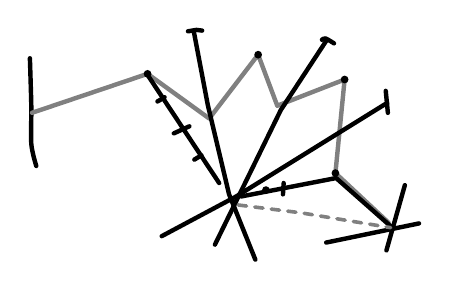
\begin{tikzpicture}[x=0.009cm,y=-0.009cm,line cap=round,line join=round]
\draw[line width=1.6pt] plot[smooth] coordinates {(6,45) (8,113) (8,166) (15,197)};
\draw[gray,line width=1.6pt] (9,122)--(172,67)--(259,130)--(328,40)--(355,112)--(450,75)--(437,207)--(512,277);
\draw[line width=1.6pt] (171,67)--(273,221);
\draw[line width=1.6pt] (186,106)--(196,100);
\draw[line width=1.6pt] (209,151)--(231,141);
\draw[line width=1.6pt] (238,188)--(248,182);
\draw[line width=1.6pt] (229,7)--(241,5)--(249,6);
\draw[line width=1.6pt] (237,6)--(257,111)--(287,237)--(324,329);
\draw[line width=1.6pt] plot[smooth] coordinates {(418,19) (423,17) (435,24)};
\draw[line width=1.6pt] (425,19)--(360,118)--(267,308);
\draw[line width=1.6pt] (192,296)--(297,240)--(510,108);
\draw[line width=1.6pt] (508,91)--(511,122);
\draw[line width=1.6pt] (304,240)--(438,214)--(515,282);
\draw[line width=1.6pt] (535,224)--(509,316);
\draw[line width=1.6pt] (424,305)--(555,278);
\draw[gray,line width=1.3pt,dashed] (300,252)--(388,263)--(515,284);
\draw[line width=1.6pt] (364,221)--(363,237);
\fill[black] (172,67) circle [radius=1.4pt];
\fill[black] (328,40) circle [radius=1.4pt];
\fill[black] (450,75) circle [radius=1.4pt];
\fill[black] (437,207) circle [radius=1.4pt];
\fill[black] (339,231) circle [radius=1.4pt];
\end{tikzpicture}}

\figure{\begin{tikzpicture}[x=0.006cm,y=-0.006cm,line cap=round,line join=round]
\draw[thin] plot[smooth] coordinates {(170,0) (105,127) (48,272) (10,430) (5,598) (29,744)};
\end{tikzpicture}}

\figure{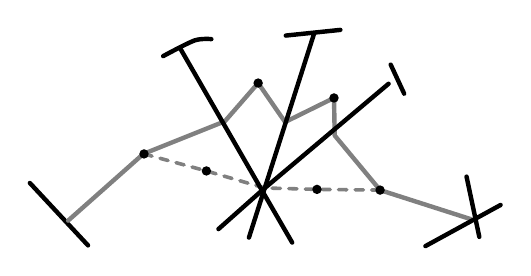
\begin{tikzpicture}[x=0.009cm,y=-0.009cm,line cap=round,line join=round]
\draw[line width=1.6pt] (0,224)--(82,312);
\draw[gray,line width=1.6pt] (54,277)--(160,183)--(275,137)--(322,83)--(360,138)--(429,104)--(430,157)--(494,234)--(622,275);
\draw[gray,line width=1.3pt,dashed] (161,183)--(249,207)--(331,231)--(405,233)--(494,234);
\draw[line width=1.6pt] plot[smooth] coordinates {(188,45) (232,23) (256,21)};
\draw[line width=1.6pt] (212,34)--(326,232)--(370,308);
\draw[line width=1.6pt] (361,16)--(438,8);
\draw[line width=1.6pt] (401,13)--(309,301);
\draw[line width=1.6pt] (266,289)--(328,234)--(506,84);
\draw[line width=1.6pt] (509,57)--(528,98);
\draw[line width=1.6pt] (558,313)--(664,255);
\draw[line width=1.6pt] (616,215)--(634,300);
\fill[black] (161,183) circle [radius=1.7pt];
\fill[black] (249,207) circle [radius=1.7pt];
\fill[black] (322,83) circle [radius=1.7pt];
\fill[black] (429,104) circle [radius=1.7pt];
\fill[black] (405,233) circle [radius=1.7pt];
\fill[black] (494,234) circle [radius=1.7pt];
\end{tikzpicture}}

\scanpage{54}
% archive sheet number: 53

\uline{\unsure{Réécrit|Récrit}} sans utiliser la partition des arcs critiques, pour déterminer les signes \deleted{de} $\varepsilon_{F'}(\deleted{\unsure{F}}a')$, quand on connaît \deleted{les $x'$ de} \inserted{les signes} $\varepsilon_F(a)$.

\uline{Proposition} \deleted{Considérons l'ens \deleted{\illegible{1}} $V_F$ (``verts'') des sommets d'ordre 4 incidents à $F$, et l'ens $\sigma_a^{F'}(V_{F'})$ (où $F'$ est la face incidente à $F$ le long de la grande arête $a$ de $\partial F$). \deleted{Soit \illegible{1}} Ces deux deux décomp. en arêtes de $\partial F$ ne \deleted{\unsure{que des}} \deleted{\unsure{ont, considérons}} \inserted{arêtes} considérons les (ferm\unsure{ées}) $\alpha$,}

Soit $A_{F,a}=$ \deleted{\unsure{$K$}} la réunion des grandes arêtes \inserted{$\alpha$} sur $F$ qui sont telles que $\sigma_a(\unsure{\alpha|a})$ soit une grande arête de $F'=\sigma_a(F)$ \unsure{à} (NB $a$ est une grande arête de $F$) Alors

a) $A$ est un arc sur $\partial F$, soit $B$ l'arc ``complémentaire''. \deleted{Alors} Considérons la subdivision de $B$ en grandes arêtes (sommets verts clairs) et en ``grandes arêtes pour $F'$'' (sommets verts foncés). Alors le nb d'arêtes $n_a(F)$ et $n_a(F')$ qui interviennent est \deleted{\unsure{ég}} compris entre 3 et 5 --- les possibilités sont (modulo échange de $F$ et $F'$) $(3,2),(3,3),(3,4)$ \deleted{Dans le} \deleted{\unsure{cas}} (cas 1) 2) 3)) --- et dans tous les cas, c'est la face spéciale qui donne lieu à 3 arcs (ce qui suffit à la déterminer, quand on est dans le cas $1^\circ$ ou $3^\circ$). De plus, on a

b) Si $\alpha$ est une \deleted{petite} arête \deleted{de} $F$ dans $A$, \deleted{\unsure{alors|al}} \deleted{alors} et $\alpha\ne a$, on a $\varepsilon_{F'}(a)=\varepsilon_F(a)$

[NB si $\alpha=a$, on a $\varepsilon_{F'}(a)=-\varepsilon_F(a)$]

c) On a les \deleted{\unsure{poss}} trois cas suivants \deleted{\unsure{fig}} pour la distribution des grandes arêtes sur $B$ (à échange près de $F$ et $F'$) et les signes correspondants

\figure{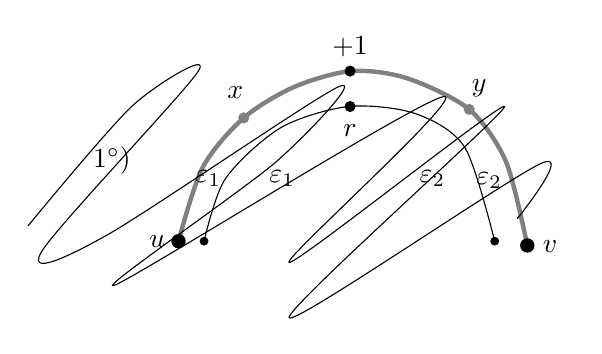
\begin{tikzpicture}[x=0.018cm,y=-0.018cm,line cap=round,line join=round]
\draw[gray,line width=1.6pt] plot[smooth] coordinates {(0,135) (17,83) (46,48) (82,26) (122,15) (161,20) (205,42) (231,79) (246,138)};
\fill[black] (0,135) circle [radius=2.6pt];
\fill[black] (246,138) circle [radius=2.6pt];
\fill[gray] (46,48) circle [radius=2pt];
\fill[gray] (205,42) circle [radius=2pt];
\node at (-47,78) {$1^\circ)$};
\node at (-15,135) {$u$};
\node at (262,139) {$v$};
\node at (40,30) {$x$};
\node at (212,27) {$y$};
\draw[thin] plot[smooth] coordinates {(18,135) (33,91) (72,55) (120,40) (167,45) (202,69) (223,135)};
\fill[black] (18,135) circle [radius=1.6pt];
\fill[black] (223,135) circle [radius=1.6pt];
\node at (21,91) {$\varepsilon_1$};
\node at (219,92) {$\varepsilon_2$};
\node at (73,91) {$\varepsilon_1$};
\node at (179,91) {$\varepsilon_2$};
\fill[black] (121,40) circle [radius=2pt];
\fill[black] (121,15) circle [radius=2pt];
\node at (121,57) {$r$};
\node at (121,-2) {$+1$};
\draw[thin] plot[smooth] coordinates {(-106,124) (-32,39) (14,15) (-97,143) (-51,131) (113,26) (70,78) (-45,166) (187,33) (78,150) (230,40) (78,189) (256,80) (239,119)};
\end{tikzpicture}}

\figure{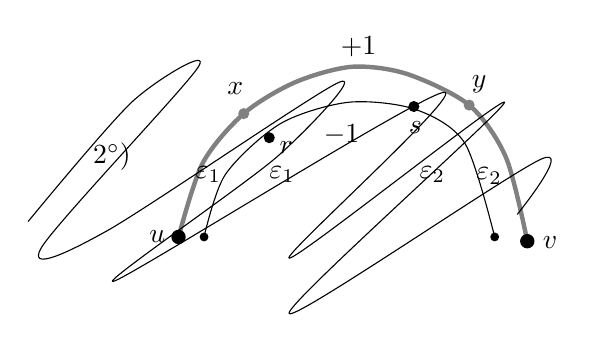
\begin{tikzpicture}[x=0.018cm,y=-0.018cm,line cap=round,line join=round]
\draw[gray,line width=1.6pt] plot[smooth] coordinates {(0,135) (17,83) (46,48) (82,26) (122,15) (161,20) (205,42) (231,79) (246,138)};
\fill[black] (0,135) circle [radius=2.6pt];
\fill[black] (246,138) circle [radius=2.6pt];
\fill[gray] (46,48) circle [radius=2pt];
\fill[gray] (205,42) circle [radius=2pt];
\node at (-47,78) {$2^\circ)$};
\node at (-15,135) {$u$};
\node at (262,139) {$v$};
\node at (40,30) {$x$};
\node at (212,27) {$y$};
\draw[thin] plot[smooth] coordinates {(18,135) (33,91) (72,55) (120,40) (167,45) (202,69) (223,135)};
\fill[black] (18,135) circle [radius=1.6pt];
\fill[black] (223,135) circle [radius=1.6pt];
\node at (21,91) {$\varepsilon_1$};
\node at (219,92) {$\varepsilon_2$};
\node at (73,91) {$\varepsilon_1$};
\node at (179,91) {$\varepsilon_2$};
\fill[black] (64,65) circle [radius=2pt];
\fill[black] (166,43) circle [radius=2pt];
\node at (76,72) {$r$};
\node at (167,58) {$s$};
\node at (115,63) {$-1$};
\node at (127,1) {$+1$};
\draw[thin] plot[smooth] coordinates {(-106,124) (-32,39) (14,15) (-97,143) (-51,131) (113,26) (70,78) (-45,166) (187,33) (78,150) (230,40) (78,189) (256,80) (239,119)};
\end{tikzpicture}}

\figure{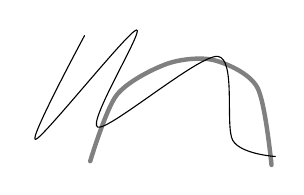
\begin{tikzpicture}[x=0.012cm,y=-0.012cm,line cap=round,line join=round]
\draw[gray,line width=1.6pt] plot[smooth] coordinates {(0,115) (28,45) (81,12) (131,8) (177,37) (192,119)};
\draw[thin] plot[smooth] coordinates {(-6,-18) (-58,92) (49,-24) (8,79) (135,4) (151,93) (196,110)};
\end{tikzpicture}}

\figure{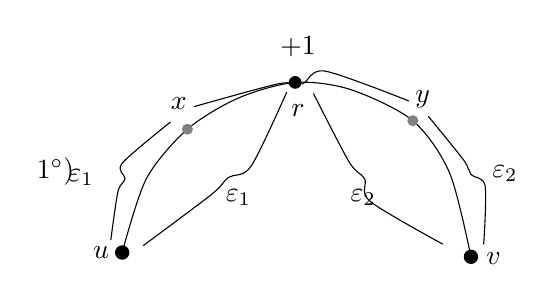
\begin{tikzpicture}[x=0.018cm,y=-0.018cm,line cap=round,line join=round]
\draw[thin] plot[smooth] coordinates {(0,135) (17,83) (46,48) (82,26) (122,15) (161,20) (205,42) (231,79) (246,138)};
\fill[black] (0,135) circle [radius=2.6pt];
\fill[black] (246,138) circle [radius=2.6pt];
\fill[gray] (46,48) circle [radius=2pt];
\fill[gray] (205,42) circle [radius=2pt];
\node at (-47,78) {$1^\circ)$};
\node at (-15,135) {$u$};
\node at (262,139) {$v$};
\node at (40,30) {$x$};
\node at (212,27) {$y$};
\draw[thin] plot[smooth] coordinates {(-8,126) (-3,92) (2,83) (0,72) (34,43)};
\node at (-29,82) {$\varepsilon_1$};
\draw[thin] plot[smooth] coordinates {(216,39) (241,70) (246,80) (256,88) (255,129)};
\node at (270,79) {$\varepsilon_2$};
\draw[thin] plot[smooth] coordinates {(51,32) (110,16) (127,16) (143,7) (202,28)};
\node at (124,-10) {$+1$};
\fill[black] (122,15) circle [radius=2.3pt];
\node at (124,35) {$r$};
\draw[thin] plot[smooth] coordinates {(15,130) (63,94) (75,82) (91,74) (116,22)};
\node at (82,96) {$\varepsilon_1$};
\draw[thin] plot[smooth] coordinates {(135,23) (160,71) (171,83) (175,99) (226,129)};
\node at (170,96) {$\varepsilon_2$};
\end{tikzpicture}}

\figure{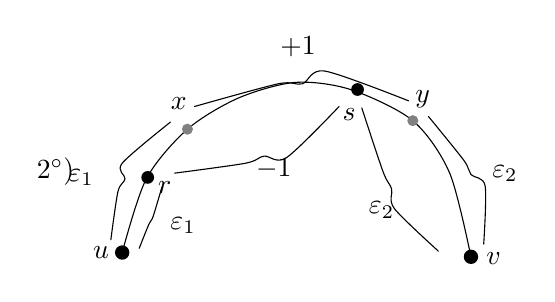
\begin{tikzpicture}[x=0.018cm,y=-0.018cm,line cap=round,line join=round]
\draw[thin] plot[smooth] coordinates {(0,135) (17,83) (46,48) (82,26) (122,15) (161,20) (205,42) (231,79) (246,138)};
\fill[black] (0,135) circle [radius=2.6pt];
\fill[black] (246,138) circle [radius=2.6pt];
\fill[gray] (46,48) circle [radius=2pt];
\fill[gray] (205,42) circle [radius=2pt];
\node at (-47,78) {$2^\circ)$};
\node at (-15,135) {$u$};
\node at (262,139) {$v$};
\node at (40,30) {$x$};
\node at (212,27) {$y$};
\draw[thin] plot[smooth] coordinates {(-8,126) (-3,92) (2,83) (0,72) (34,43)};
\node at (-29,82) {$\varepsilon_1$};
\draw[thin] plot[smooth] coordinates {(216,39) (241,70) (246,80) (256,88) (255,129)};
\node at (270,79) {$\varepsilon_2$};
\draw[thin] plot[smooth] coordinates {(51,32) (110,16) (127,16) (143,7) (202,28)};
\node at (124,-10) {$+1$};
\fill[black] (18,82) circle [radius=2.3pt];
\fill[black] (166,20) circle [radius=2.3pt];
\node at (30,89) {$r$};
\node at (160,38) {$s$};
\draw[thin] plot[smooth] coordinates {(12,132) (18,117) (20,113) (22,109) (28,89)};
\node at (43,116) {$\varepsilon_1$};
\draw[thin] plot[smooth] coordinates {(37,79) (87,72) (100,67) (116,68) (153,32)};
\node at (107,76) {$-1$};
\draw[thin] plot[smooth] coordinates {(169,33) (184,78) (190,90) (192,104) (223,134)};
\node at (183,105) {$\varepsilon_2$};
\end{tikzpicture}}

\figure{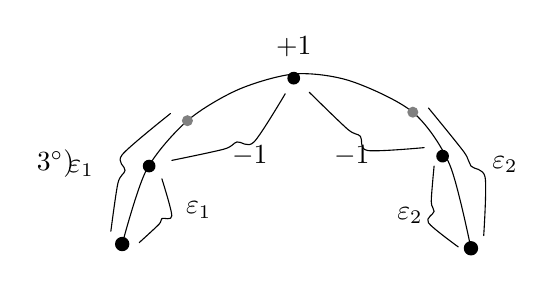
\begin{tikzpicture}[x=0.018cm,y=-0.018cm,line cap=round,line join=round]
\draw[thin] plot[smooth] coordinates {(0,135) (17,83) (46,48) (82,26) (122,15) (161,20) (205,42) (231,79) (246,138)};
\fill[black] (0,135) circle [radius=2.6pt];
\fill[black] (246,138) circle [radius=2.6pt];
\fill[gray] (46,48) circle [radius=2pt];
\fill[gray] (205,42) circle [radius=2pt];
\node at (-47,78) {$3^\circ)$};
\draw[thin] plot[smooth] coordinates {(-8,126) (-3,92) (2,83) (0,72) (34,43)};
\node at (-29,82) {$\varepsilon_1$};
\draw[thin] plot[smooth] coordinates {(216,39) (241,70) (246,80) (256,88) (255,129)};
\node at (270,79) {$\varepsilon_2$};
\fill[black] (19,80) circle [radius=2.3pt];
\fill[black] (121,18) circle [radius=2.3pt];
\fill[black] (226,73) circle [radius=2.3pt];
\node at (121,-4) {$+1$};
\draw[thin] plot[smooth] coordinates {(12,134) (26,121) (28,117) (35,115) (28,89)};
\node at (54,111) {$\varepsilon_1$};
\draw[thin] plot[smooth] coordinates {(35,76) (72,68) (81,63) (93,63) (115,29)};
\node at (90,73) {$-1$};
\draw[thin] plot[smooth] coordinates {(132,28) (159,54) (168,59) (173,69) (213,67)};
\node at (162,73) {$-1$};
\draw[thin] plot[smooth] coordinates {(220,80) (218,105) (220,112) (216,120) (237,137)};
\node at (203,115) {$\varepsilon_2$};
\end{tikzpicture}}

\scanpage{55}
% archive sheet number: 54

\uline{Corollaire} Dans tous les cas, la distribution des signes $\varepsilon_a(F)$ détermine celle des $\varepsilon_{a'}(F')$. \deleted{C'est clair \unsure{d}}

C'est clair d'abord dans les cas 1° et 3°, où on sait laquelle des faces $F,F'$ est la spécialisée de l'autre, \deleted{et par suite} Mais dans le cas \inserted{``symétrique''} 2°), \deleted{comme on connaît les signes $\varepsilon_a(F)$, on} On voit que \deleted{les} deux \inserted{grandes} arêtes extrêmes correspondantes pour $F,F'$ ont $=$ signe (c'est \unsure{tjrs} le cas, y compris dans les cas 1° et 2°), et pour les arêtes qui \inserted{ne} sont pas de ces types, elles sont (pour $F/F'$ fixé) toutes de $=$ signe (\uline{NB} leur nb, suivant les cas, est $(1,0)$, $(1,1)$ ou $(1,2)$) et les signes en question pour $F$ et pour $F'$ sont opposés.

\uline{Corollaire} Quand on connaît les signes $\varepsilon_F(a)$ pour \uline{une} face $F$, on les connaît pour \uline{ttes} (grâce à la connexité de $\mathcal X$).

J'ai supposé implicit\unsure{nt} \deleted{que} dans la vérification de la proposition que ni $F$, ni $F'$ n'est une face exceptionnelle (correspondant à une position relative exceptionnelle, i.e. ``supercritique''). Il faudrait que j'examine séparément \deleted{\unsure{de}} cas de telles faces. Pour une telle face, il n'y a que quatre grandes arêtes, et la distribution des signes est connue ---

Cela semble donner une façon simple de déduire les signes \inserted{(i.e. les \unsure{visées})} de \deleted{la} seule structure de carte de $(\mathcal X,K,S_K)$, sans avoir à utiliser les arcs critiques, et encore moins \deleted{les} le \deleted{\unsure{complexe}} graphe $L\subset\mathcal X$.

\scanpage{56}
% archive sheet number: 55

\[ (\nu_{s_1}-1)+(\nu_{s_2}-1)\ldots+(\underbrace{\nu_{s_n}}_{\nu_{s_0}}-1)\unsure{''} \]

\figure{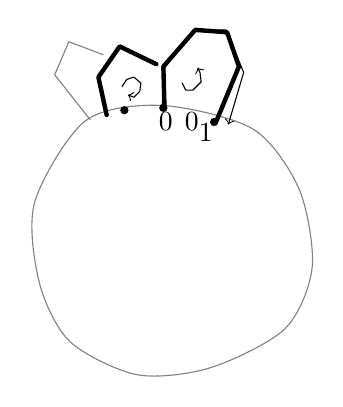
\begin{tikzpicture}[x=0.015cm,y=-0.015cm,line cap=round,line join=round]
\draw[gray,thin] plot[smooth cycle] coordinates {(95,93) (160,80) (237,100) (276,151) (287,217) (264,269) (201,302) (139,308) (82,280) (56,230) (52,162)};
\draw[gray,thin] (99,92)--(69,54)--(81,26)--(110,37);
\draw[->] (160,81)--(162,48)--(187,17)--(214,16)--(229,52)--(216,96);
\draw[line width=1.6pt] (162,83)--(161,47)--(188,16)--(215,18)--(225,47)--(206,93);
\draw[line width=1.6pt] (113,88)--(106,56)--(124,30)--(155,45);
\draw[->] (126,64)--(130,58)--(136,56)--(142,61)--(141,68)--(136,73)--(131,71);
\draw[->] (177,61)--(180,67)--(186,67)--(193,60)--(192,52)--(190,48);
\fill[black] (128,84) circle [radius=1.5pt];
\fill[black] (161,82) circle [radius=1.5pt];
\fill[black] (204,94) circle [radius=1.5pt];
\node at (163,94) {$0$};
\node at (185,94) {$0$};
\node at (197,103) {$1$};
\end{tikzpicture}}

\figure{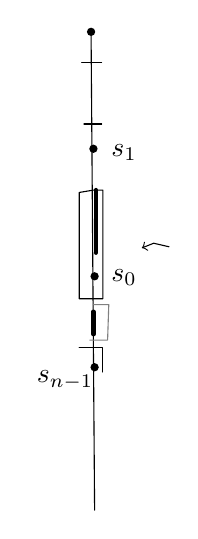
\begin{tikzpicture}[x=0.015cm,y=-0.015cm,line cap=round,line join=round]
\draw[thin] (26,0)--(29,405);
\draw[thin] (18,26)--(35,26);
\draw[thin] (20,78)--(35,78);
\fill[black] (26,0) circle [radius=1.5pt];
\fill[black] (28,99) circle [radius=1.5pt];
\fill[black] (29,207) circle [radius=1.5pt];
\fill[black] (29,284) circle [radius=1.5pt];
\draw[thin] (27,134)--(36,134)--(36,226)--(16,226)--(16,136)--(28,134);
\draw[line width=1.6pt] (30,134)--(30,187);
\draw[gray,thin] (28,231)--(41,231)--(40,261)--(25,261);
\draw[line width=1.6pt] (28,237)--(28,256);
\draw[thin] (16,267)--(36,267)--(36,288);
\node at (54,102) {$s_1$};
\node at (54,208) {$s_0$};
\node at (4,295) {$s_{n-1}$};
\draw[->] (92,182)--(79,179)--(69,183);
\end{tikzpicture}}

\[ \begin{aligned}
l_s&=\deleted{\unsure{\ell}}n-\nu_s\\
l_a&=\deleted{\unsure{\ell}}n-1-(\nu_s-1)-(\nu_t-1)\\
&=n\deleted{\unsure{+}}\unsure{-}(\nu_s+\nu_t-1)=(n-\nu_s)-(\nu_t-1)\\
l_s-l_a&=\nu_t-1\quad\deleted{\unsure{=2|=1}}\\
\chi_{2n}(s)&=\sum_{\substack{s\text{ sommets}\\\text{sur }D_i}}(\nu(s)-1)=n-1
\end{aligned} \]

\margin{multiplicité du sommet \quad $\mathbb Z/N\mathbb Z$}

\[ \lambda(t)=\widetilde\rho_p(t)=(-1)^p(t-\chi_p) \]

ici $p=2n$ donc $(-1)^p=+1$

\[ \deleted{\unsure{\beta}} \quad \deleted{\text{il faut}}\quad \lambda(t)=\deleted{\unsure{a}}t-\chi_{2n}=t-(n-1) \]

\uline{NB}

\[ \begin{aligned}
\rho_p(t)&=\sigma_{p-1}\ldots\sigma_0(t)=\deleted{(-1)^{p-1}(\chi_p-t)}\inserted{(-1)^p(t-\chi_p)}\\
&\deleted{=(-1)^p t+(-1)^{p-1}\chi_p}
\end{aligned} \]

Passage de $F_p$ à $F_0$ se fait par $t\longleftarrow\deleted{\unsure{t}}\ t$ \deleted{(\unsure{en effet}, \illegible{3})}

\[ \underbrace{\sigma_{p-1}\sigma_p\ldots\sigma_0}_{\rho_p(t)}(t)=(-1)^{p-1}\ldots \]

\figure{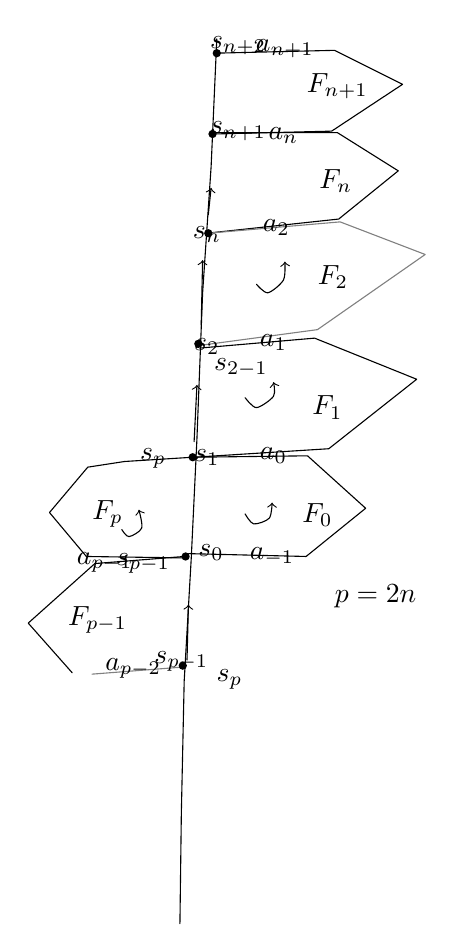
\begin{tikzpicture}[x=0.018cm,y=-0.018cm,line cap=round,line join=round]
\draw[thin] (125,0)--(121,90)--(115,179)--(111,282)--(107,366)--(102,453)--(100,546)--(99,624);
\draw[thin] (124,10)--(208,8)--(256,32)--(206,65)--(123,67);
\draw[thin] (122,66)--(210,66)--(253,93)--(211,127)--(118,137);
\draw[gray,thin] (119,137)--(212,129)--(272,152)--(196,205)--(114,216);
\draw[thin] (113,218)--(194,211)--(266,240)--(204,289)--(109,295);
\draw[thin] (109,295)--(189,294)--(230,331)--(188,365)--(105,363);
\draw[thin] (108,295)--(60,298)--(34,302)--(7,334)--(33,365)--(101,366);
\draw[thin] (102,365)--(39,370)--(-8,412)--(23,447);
\draw[gray,thin] (37,448)--(101,443);
\draw[->] (104,438)--(105,399);
\draw[->] (109,284)--(111,244);
\draw[->] (114,202)--(115,156);
\draw[->] (119,124)--(121,105);
\fill[black] (125,10) circle [radius=1.5pt];
\fill[black] (122,67) circle [radius=1.5pt];
\fill[black] (119,137) circle [radius=1.5pt];
\fill[black] (112,215) circle [radius=1.5pt];
\fill[black] (108,295) circle [radius=1.5pt];
\fill[black] (103,365) circle [radius=1.5pt];
\fill[black] (101,442) circle [radius=1.5pt];
\node at (140,5) {$s_{n+2}$};
\node at (173,7) {$a_{n+1}$};
\node at (210,33) {$F_{n+1}$};
\node at (140,65) {$s_{n+1}$};
\node at (172,68) {$a_n$};
\node at (209,100) {$F_n$};
\node at (118,138) {$s_n$};
\node at (167,133) {$a_2$};
\node at (207,168) {$F_2$};
\node at (118,217) {$s_2$};
\node at (142,232) {$s_{2-1}$};
\node at (165,214) {$a_1$};
\node at (203,260) {$F_1$};
\node at (118,295) {$s_1$};
\node at (80,296) {$s_p$};
\node at (165,294) {$a_0$};
\node at (196,336) {$F_0$};
\node at (48,335) {$F_p$};
\node at (73,370) {$s_{p-1}$};
\node at (121,362) {$s_0$};
\node at (164,365) {$a_{-1}$};
\node at (46,369) {$a_{p-1}$};
\node at (41,410) {$F_{p-1}$};
\node at (66,444) {$a_{p-2}$};
\node at (100,439) {$s_{p-1}$};
\node at (134,452) {$\deleted{\unsure{s_p}}$};
\node at (237,393) {$p=2n$};
\draw[->] plot[smooth] coordinates {(58,346) (63,351) (72,345) (70,332)};
\draw[->] plot[smooth] coordinates {(145,335) (151,342) (162,338) (164,327)};
\draw[->] plot[smooth] coordinates {(145,253) (153,260) (165,252) (165,242)};
\draw[->] plot[smooth] coordinates {(153,173) (161,179) (172,170) (173,157)};
\end{tikzpicture}}

\figure{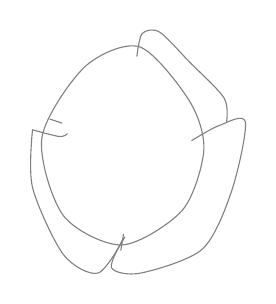
\begin{tikzpicture}[x=0.017cm,y=-0.017cm,line cap=round,line join=round]
\draw[gray,thin] plot[smooth cycle] coordinates {(16,79) (48,26) (89,11) (126,51) (137,88) (121,133) (76,159) (32,137)};
\draw[gray,thin] plot[smooth] coordinates {(9,73) (29,78) (35,76)};
\draw[gray,thin] plot[smooth] coordinates {(9,73) (9,116) (32,166) (58,180) (78,153)};
\draw[gray,thin] plot[smooth] coordinates {(77,154) (68,176) (90,180) (136,162) (158,118) (168,67) (148,70) (128,81)};
\draw[gray,thin] plot[smooth] coordinates {(154,67) (152,49) (126,22) (104,0) (91,1) (87,18)};
\draw[gray,thin] (22,65)--(31,68);
\draw[gray,thin] (77,151)--(75,163);
\end{tikzpicture}}

\figure{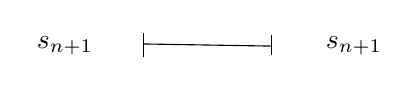
\begin{tikzpicture}[x=0.027cm,y=-0.027cm,line cap=round,line join=round]
\draw[thin] (0,2)--(60,3);
\draw[thin] (0,-3)--(0,8);
\draw[thin] (60,-2)--(60,7);
\node at (-37,3) {$s_{n+1}$};
\node at (99,3) {$s_{n+1}$};
\end{tikzpicture}}

\diagram{\begin{tikzcd}[ampersand replacement=\&,column sep=huge]
P(F_n) \arrow[r,"\sigma_{a_n}"] \arrow[d,phantom,"\unsure{\wr}" description] \& P(F_{n+1}) \arrow[d,phantom,"\unsure{\wr}" description]\\
\mathbb Z/N\mathbb Z \arrow[r,"\sigma_n"] \arrow[u,phantom,"\varphi_n"'] \& \deleted{\unsure{\mathbb Z}}\mathbb Z/N\mathbb Z \arrow[u,phantom,"\varphi_{n+1}"]
\end{tikzcd}}

$\sigma_n$ \quad \unsure{a)} respecte la structure polygonale

b) renverse l'orientation

c) transforme $\underbrace{\varphi_n^{-1}(s_{n+1})}_{l_n}$ en $\underset{\substack{\Vert\\0}}{\varphi_{n+1}^{-1}(s_{n+1})}$

\[ \text{donc}\quad \sigma_n(t)=l_n-t \]

\[ \begin{aligned}
\sigma_0(t)&=l_0-t\\
\sigma_1(t)&=l_1-t &\sigma_1\sigma_0(t)&=l_1-(l_0-t)=l_1-l_0+t\\
\sigma_2(t)&=l_2-t &\sigma_2\sigma_1\sigma_0(t)&=l_2-l_1+l_0-t
\end{aligned} \]

\[ \begin{aligned}
(\underbrace{\overbrace{\sigma_n\deleted{\unsure{\sigma}}\sigma_{n-1}\ldots\sigma_0}^{n+1\ \text{facteurs}}}_{\rho_{n+1}})(t)&=l_n-l_{n-1}-\ldots+(-1)^n l_0+(-1)^{n+1}t\\
&=(-1)^n(\chi_{n+1}-t)=(-1)^{n+1}(t-\chi_{n+1})\\
\text{où}\quad \chi_{n+1}&=\underbrace{l_0\deleted{+}l_1-\ldots+(-1)^n l_n}_{n+1\ \text{termes}}
\end{aligned} \]

\scanpage{57}
% archive sheet number: 56

% printed form
\texttt{//*\quad CRAY2\quad 0296\qquad \unsure{I|1}}

{\scriptsize
\begin{verbatim}
           00000000      00000000     555555555555       11
         0000000000    0000000000    555555555555       111
       00      0000  00      0000   55                 1111
      00     00 00  00     00 00   55                  11
     00    00  00  00    00  00   55                  11
    00   00   00  00   00   00   555555555           11
   00  00    00  00  00    00   555555555           11
  00 00     00  00 00     00           55          11
 0000      00  0000      00           55          11
000       00  000       00           55          11
0000000000    0000000000   555555555555   1111111111
00000000      00000000    55555555555    1111111111
\end{verbatim}
}

{\scriptsize\begin{verbatim}
 CCCCCCCCCC   RRRRRRRRRRR    AAAAAAAAAA   YY        YY   2222222222
CCCCCCCCCCCC  RRRRRRRRRRRR  AAAAAAAAAAAA  YY        YY  222222222222
CC        CC  RR        RR  AA        AA   YY      YY   22        22
CC            RR        RR  AA        AA    YY    YY              22
CC            RR        RR  AA        AA     YY  YY               22
CC            RRRRRRRRRRRR  AAAAAAAAAAAA      YYYY               22
CC            RRRRRRRRRRR   AAAAAAAAAAAA       YY              22
CC            RR    RR      AA        AA       YY            22
CC            RR     RR     AA        AA       YY          22
CC        CC  RR      RR    AA        AA       YY        22
CCCCCCCCCCCC  RR       RR   AA        AA       YY       222222222222
 CCCCCCCCCC   RR        RR  AA        AA       YY       222222222222
\end{verbatim}
}

{\fontsize{4.5}{5.9}\selectfont
\begin{verbatim}
****A  START  JOB  296  CRAY2                           ROOM        5.00.32 PM 17 AUG 82  R6.PR1    SYS JES2  JOB  296  START  A****
****A  START  JOB  296  CRAY2                           ROOM        5.00.32 PM 17 AUG 82  R6.PR1    SYS JES2  JOB  296  START  A****
****A  START  JOB  296  CRAY2                           ROOM        5.00.32 PM 17 AUG 82  R6.PR1    SYS JES2  JOB  296  START  A****
****A  START  JOB  296  CRAY2                           ROOM        5.00.32 PM 17 AUG 82  R6.PR1    SYS JES2  JOB  296  START  A****
****A  START  JOB  296  CRAY2                           ROOM        5.00.32 PM 17 AUG 82  R6.PR1    SYS JES2  JOB  296  START  A****
****A  START  JOB  296  CRAY2                           ROOM        5.00.32 PM 17 AUG 82  R6.PR1    SYS JES2  JOB  296  START  A****
\end{verbatim}
}

\texttt{DERNIERE MISE A JOUR DE JOURNAL : 11-08-82}\\
\texttt{ARRET DE L'ORDINATEUR LE MERCREDI 18 AOUT DE 7 H A 8 H.}\\
\texttt{ATTENTION .........}

\texttt{] \qquad UN ARRET EXCEPTIONNEL POUR PREPARER L'ARRIVEE DE NOUVELLES}\\
\texttt{] \qquad UNITES AURA LIEU DU VENDREDI 20 AOUT A 17H 30 AU LUNDI}\\
\texttt{] \qquad 23 AOUT A 8H.}

\[ \handwritten{\begin{aligned}\nu(\underset{2}{\underbrace{n-1}})+\nu(n-3)&=2\nu n-4\nu\deleted{=\unsure{2\nu(n-1)}}\\
&\deleted{=\nu(2n-3)}\\
&=\boxed{2\nu(n-2)}
\end{aligned}} \]

\figure{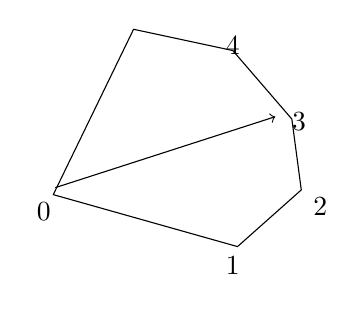
\begin{tikzpicture}[x=0.03cm,y=-0.03cm,line cap=round,line join=round]
\draw[thin] (0,70)--(34,0)--(76,9)--(101,38)--(105,68)--(78,92)--(0,70);
\draw[->] (1,67)--(94,37);
\node at (-4,77) {$0$};
\node at (76,100) {$1$};
\node at (113,75) {$2$};
\node at (104,39) {$3$};
\node at (76,7) {$4$};
\end{tikzpicture}}

\figure{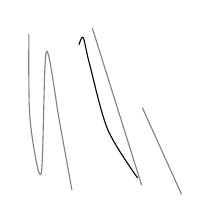
\begin{tikzpicture}[x=0.013cm,y=-0.013cm,line cap=round,line join=round]
\draw[gray,thin] plot[smooth] coordinates {(1,40) (2,122) (13,176) (18,57) (31,126) (43,192)};
\draw[thin] plot[smooth] coordinates {(50,50) (54,43) (60,68) (78,133) (107,180)};
\draw[gray,thin] (63,34)--(111,187);
\draw[gray,thin] (112,112)--(150,196);
\end{tikzpicture}}

\figure{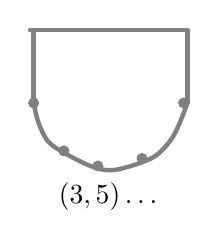
\begin{tikzpicture}[x=0.016cm,y=-0.016cm,line cap=round,line join=round]
\draw[gray,line width=1.6pt] (0,0)--(125,0)--(125,58);
\draw[gray,line width=1.6pt] (3,0)--(3,58);
\draw[gray,line width=1.6pt] plot[smooth] coordinates {(3,58) (7,74) (17,91) (48,108) (68,111) (98,101) (114,84) (125,58)};
\fill[gray] (3,58) circle [radius=2pt];
\fill[gray] (122,58) circle [radius=2pt];
\fill[gray] (27,96) circle [radius=2pt];
\fill[gray] (54,108) circle [radius=2pt];
\fill[gray] (89,102) circle [radius=2pt];
\node at (62,132) {$(3,5)\ldots$};
\end{tikzpicture}}

\figure{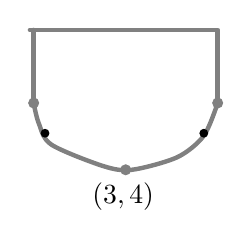
\begin{tikzpicture}[x=0.016cm,y=-0.016cm,line cap=round,line join=round]
\draw[gray,line width=1.6pt] (0,0)--(149,0)--(149,58);
\draw[gray,line width=1.6pt] (3,0)--(3,58);
\draw[gray,line width=1.6pt] plot[smooth] coordinates {(3,58) (7,74) (17,91) (58,108) (81,111) (117,101) (138,84) (149,58)};
\fill[gray] (3,58) circle [radius=2pt];
\fill[gray] (149,58) circle [radius=2pt];
\fill[gray] (76,111) circle [radius=2pt];
\fill[black] (12,82) circle [radius=1.6pt];
\fill[black] (138,82) circle [radius=1.6pt];
\node at (74,132) {$(3,4)$};
\end{tikzpicture}}

\figure{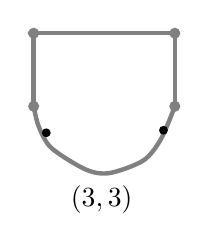
\begin{tikzpicture}[x=0.016cm,y=-0.016cm,line cap=round,line join=round]
\draw[gray,line width=1.6pt] (0,0)--(115,0)--(115,58);
\draw[gray,line width=1.6pt] (3,0)--(3,58);
\draw[gray,line width=1.6pt] plot[smooth] coordinates {(3,58) (7,74) (17,91) (44,108) (63,111) (90,101) (104,84) (115,58)};
\fill[gray] (3,0) circle [radius=2pt];
\fill[gray] (3,58) circle [radius=2pt];
\fill[gray] (115,0) circle [radius=2pt];
\fill[gray] (115,58) circle [radius=2pt];
\fill[black] (13,79) circle [radius=1.6pt];
\fill[black] (106,77) circle [radius=1.6pt];
\node at (57,132) {$(3,3)$};
\end{tikzpicture}}

\handwritten{$2(\deleted{\unsure{n-2\nu}})$}

\figure{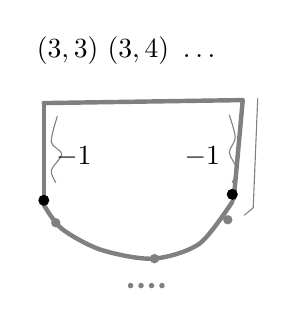
\begin{tikzpicture}[x=0.019cm,y=-0.019cm,line cap=round,line join=round]
\draw[gray,line width=1.6pt] (0,0)--(133,-2)--(127,64);
\draw[gray,line width=1.6pt] (0,0)--(0,68);
\draw[gray,line width=1.6pt] plot[smooth] coordinates {(0,68) (12,84) (38,98) (73,104) (104,94) (126,66)};
\draw[gray,thin] plot[smooth] coordinates {(9,9) (5,26) (12,34) (5,45) (8,53)};
\draw[gray,thin] plot[smooth] coordinates {(124,8) (128,23) (124,33) (129,44) (126,53)};
\draw[gray,thin] (143,-3)--(140,70)--(134,75);
\fill[black] (0,65) circle [radius=2pt];
\fill[black] (126,61) circle [radius=2pt];
\fill[gray] (8,80) circle [radius=1.7pt];
\fill[gray] (74,104) circle [radius=1.7pt];
\fill[gray] (123,78) circle [radius=1.7pt];
\fill[gray] (58,122) circle [radius=1pt];
\fill[gray] (65,122) circle [radius=1pt];
\fill[gray] (72,122) circle [radius=1pt];
\fill[gray] (79,122) circle [radius=1pt];
\node at (20,36) {$-1$};
\node at (106,36) {$-1$};
\node at (55,-35) {$(3,3)\ (3,4)\ \ldots$};
\end{tikzpicture}}

\figure{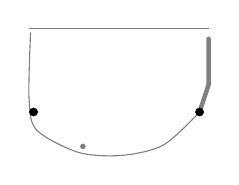
\begin{tikzpicture}[x=0.019cm,y=-0.019cm,line cap=round,line join=round]
\draw[gray,thin] (0,0)--(120,0);
\draw[gray,line width=1.6pt] (120,7)--(120,38)--(114,56);
\draw[gray,thin] plot[smooth] coordinates {(1,3) (0,47) (5,68) (33,83) (62,85) (90,78) (115,55)};
\fill[black] (3,56) circle [radius=1.6pt];
\fill[black] (114,56) circle [radius=1.6pt];
\fill[gray] (36,79) circle [radius=1pt];
\end{tikzpicture}}

\figure{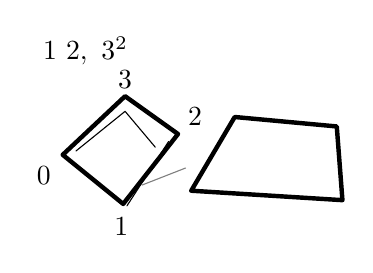
\begin{tikzpicture}[x=0.024cm,y=-0.024cm,line cap=round,line join=round]
\draw[line width=1.6pt] (0,31)--(33,0)--(61,20)--(32,57)--(0,31);
\draw[thin] (7,29)--(33,8)--(49,27);
\draw[thin] (56,24)--(34,58);
\draw[line width=1.6pt] (68,50)--(91,11)--(145,16)--(148,55)--(68,50);
\draw[gray,thin] (42,47)--(65,38);
\node at (-10,42) {$0$};
\node at (31,69) {$1$};
\node at (70,11) {$2$};
\node at (33,-9) {$3$};
\node at (12,-24) {$1\ 2,\ 3^{\unsure{2}}$};
\end{tikzpicture}}

\figure{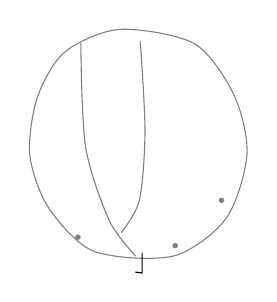
\begin{tikzpicture}[x=0.012cm,y=-0.012cm,line cap=round,line join=round]
\draw[gray,thin] plot[smooth cycle] coordinates {(40,33) (98,9) (177,24) (219,78) (233,141) (211,209) (155,249) (71,244) (23,198) (3,142) (11,81)};
\draw[gray,thin] plot[smooth] coordinates {(57,24) (62,133) (87,211) (115,249)};
\draw[gray,thin] plot[smooth] coordinates {(120,22) (125,117) (119,190) (100,224)};
\fill[gray] (54,229) circle [radius=1pt];
\fill[gray] (157,238) circle [radius=1pt];
\fill[gray] (206,190) circle [radius=1pt];
\draw[thin] (122,246)--(122,267)--(115,266);
\end{tikzpicture}}

\figure{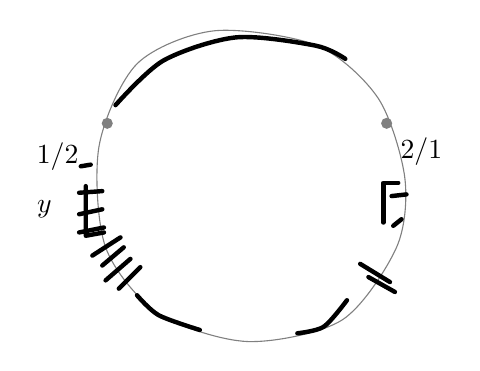
\begin{tikzpicture}[x=0.021cm,y=-0.021cm,line cap=round,line join=round]
\draw[gray,thin] plot[smooth cycle] coordinates {(12,71) (35,21) (82,1) (144,10) (181,42) (197,90) (192,132) (159,176) (102,189) (48,172) (16,132)};
\draw[line width=1.6pt] plot[smooth] coordinates {(22,46) (51,19) (95,5) (143,10) (161,18)};
\draw[line width=1.6pt] (1,83)--(7,82);
\draw[line width=1.6pt] (4,95)--(4,125)--(15,123);
\draw[line width=1.6pt] (0,99)--(14,98);
\draw[line width=1.6pt] (0,112)--(14,109);
\draw[line width=1.6pt] (0,123)--(15,120);
\draw[line width=1.6pt] (8,137)--(25,126);
\draw[line width=1.6pt] (14,143)--(27,132);
\draw[line width=1.6pt] (16,152)--(31,139);
\draw[line width=1.6pt] (24,157)--(37,144);
\draw[line width=1.6pt] plot[smooth] coordinates {(35,161) (48,173) (73,182)};
\draw[line width=1.6pt] plot[smooth] coordinates {(132,184) (148,180) (162,164)};
\draw[line width=1.6pt] (175,150)--(191,159);
\draw[line width=1.6pt] (170,142)--(188,153);
\draw[line width=1.6pt] (184,117)--(184,93)--(193,93);
\draw[line width=1.6pt] (190,119)--(195,115);
\draw[line width=1.6pt] (189,101)--(198,100);
\fill[gray] (17,57) circle [radius=2pt];
\fill[gray] (186,57) circle [radius=2pt];
\node at (-13,77) {$\unsure{1/2}$};
\node at (207,74) {$\unsure{2/1}$};
\node at (-21,109) {$\unsure{y}$};
\end{tikzpicture}}

\figure{\begin{tikzpicture}[x=0.018cm,y=-0.018cm,line cap=round,line join=round]
\draw[gray,thin] plot[smooth] coordinates {(45,0) (50,52) (29,117) (1,188) (36,172) (76,144) (72,158)};
\draw[gray,thin] (6,282)--(0,299);
\end{tikzpicture}}

\figure{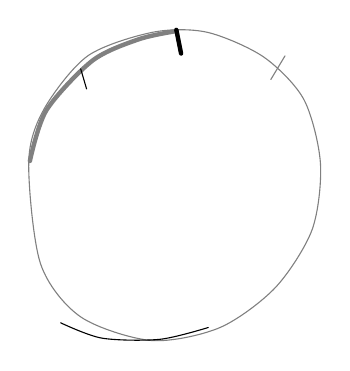
\begin{tikzpicture}[x=0.015cm,y=-0.015cm,line cap=round,line join=round]
\draw[gray,thin] plot[smooth cycle] coordinates {(5,118) (18,73) (55,28) (110,8) (156,8) (204,29) (238,65) (252,119) (245,175) (214,224) (167,258) (109,269) (49,249) (15,204)};
\draw[gray,line width=1.6pt] plot[smooth] coordinates {(6,117) (20,74) (59,32) (98,14) (130,7)};
\draw[line width=1.6pt] (130,6)--(134,26);
\draw[thin] (49,39)--(54,56);
\draw[gray,thin] (210,48)--(222,28);
\draw[thin] plot[smooth] coordinates {(32,254) (67,267) (116,268) (157,258)};
\end{tikzpicture}}

\figure{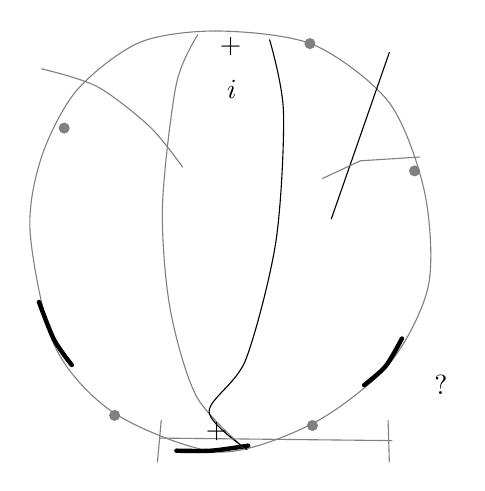
\begin{tikzpicture}[x=0.016cm,y=-0.016cm,line cap=round,line join=round]
\draw[gray,thin] plot[smooth cycle] coordinates {(1,160) (10,100) (38,47) (88,9) (151,0) (226,11) (286,57) (314,128) (317,202) (286,264) (226,311) (151,334) (69,304) (21,251)};
\draw[line width=1.6pt] plot[smooth] coordinates {(8,215) (20,245) (34,265)};
\draw[line width=1.6pt] plot[smooth] coordinates {(266,281) (283,266) (296,244)};
\draw[line width=1.6pt] plot[smooth] coordinates {(117,333) (145,333) (174,329)};
\draw[gray,thin] plot[smooth] coordinates {(134,3) (117,42) (106,139) (112,220) (133,290) (172,332)};
\draw[thin] plot[smooth] coordinates {(191,7) (202,64) (196,167) (172,261) (143,302) (173,332)};
\draw[gray,thin] (104,323)--(288,325);
\draw[gray,thin] (105,309)--(102,342);
\draw[gray,thin] (285,309)--(286,342);
\draw[gray,thin] plot[smooth] coordinates {(10,30) (54,44) (96,76) (122,108)};
\draw[thin] (240,149)--(286,17);
\draw[gray,thin] (233,117)--(263,103)--(310,100);
\fill[gray] (28,77) circle [radius=2pt];
\fill[gray] (223,10) circle [radius=2pt];
\fill[gray] (306,111) circle [radius=2pt];
\fill[gray] (225,313) circle [radius=2pt];
\fill[gray] (68,305) circle [radius=2pt];
\node at (160,12) {$+$};
\node at (161,46) {$\unsure{i}$};
\node at (149,318) {$\unsure{+}$};
\node at (327,281) {$\unsure{?}$};
\end{tikzpicture}}

\figure{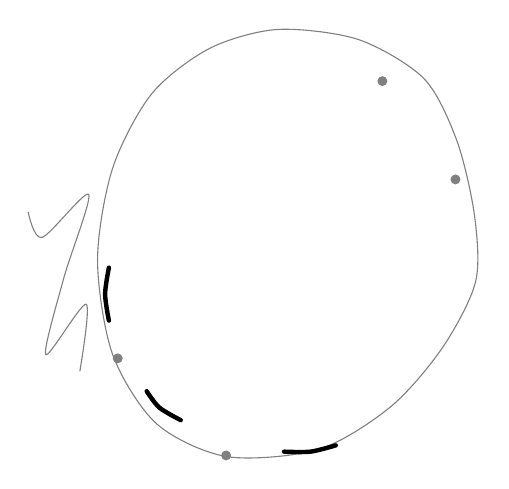
\begin{tikzpicture}[x=0.016cm,y=-0.016cm,line cap=round,line join=round]
\draw[gray,thin] plot[smooth cycle] coordinates {(1,183) (13,110) (44,51) (90,15) (144,0) (208,8) (260,39) (286,88) (300,147) (301,200) (275,252) (234,299) (177,333) (104,339) (48,313) (13,258)};
\draw[line width=1.6pt] plot[smooth] coordinates {(10,189) (7,210) (10,231)};
\draw[line width=1.6pt] plot[smooth] coordinates {(40,287) (50,300) (67,310)};
\draw[line width=1.6pt] plot[smooth] coordinates {(149,335) (170,335) (190,330)};
\draw[gray,thin] plot[smooth] coordinates {(-54,145) (-43,165) (-6,131) (-26,198) (-40,258) (-8,218) (-13,271)};
\fill[gray] (227,41) circle [radius=1.8pt];
\fill[gray] (285,119) circle [radius=1.8pt];
\fill[gray] (17,261) circle [radius=1.8pt];
\fill[gray] (103,338) circle [radius=1.8pt];
\end{tikzpicture}}

\scanpage{58}
% archive sheet number: 57

3.1.84

Transport parallèle le long d'un demi-tour, \deleted{\unsure{au}} le long d'une position relative \deleted{singulière de position} supersingulière

\[ \boxed{\lambda(t)=t-(n-1)} \]

\uline{NB} Le pgcd de $n-1$ et de $2n$ est 1 si $n$ pair, 2 si $n$ impair.

% slanted
\margin{\unsure{Toute|Tout} la suite \unsure{couillon|couill.} !}

\deleted{Donc on voit que l'image de
\[ \Pi_1(\mathcal X)\longrightarrow\deleted{\unsure{\mathbb Z}}\mathbb D_{2n} \]
a une image qui contient $\mathbb D_{2n}^{+}\inserted{\simeq\mathbb Z/n\mathbb Z}$ si $n$ pair (donc cette image est d'indice 1 ou 2) \deleted{ou bien elle} et elle contient $\mathbb Z/n\mathbb Z$ si $n$ impair (donc elle est alors d'indice 1, 2 ou 4)

\deleted{Cela ne nous dit rien sur les compos} Si on prend le dédoublage $\widetilde{\mathcal X}$ de $\mathcal X$ suivant les composantes supersingulières de $K$, on trouve dans l'image de
\[ \Pi_1(\widetilde{\mathcal X})\longrightarrow\mathbb D_{2n} \]
les éléments
\[ t\longrightarrow\lambda'(t)=t-2(n-1). \]
Or le pgcd de $2(n-1)$ et $n$ est \unsure{tjrs} 2. Donc l'image contient \unsure{tjrs} $\mathbb Z/n\mathbb Z$, d'indice 4}

(le quotient étant $\mathbb D_2\simeq\mathbb F_2\times\mathbb F_2$)

\deleted{Ceci ne nous dit \inserted{rien} sur l'image de $\Pi_1(\mathcal X)$ \unsure{ou} $\Pi_1(\widetilde{\mathcal X})$ dans $\mathbb D_2$, et en particulier sur son image dans $\pm1$, \inserted{par la} \unsure{composée} avec
\[ \mathbb D_{2n}\xrightarrow{\chi}\pm1 \]}

\deleted{On a l'impression que pour avoir des informations, il faut faire pivoter un \unsure{piv.} autour d'un sommet de $\underline{\Sigma}$ et faire ainsi un cycle et voir l'effet produit. On va faire un demi-tour, à partir d'une position supersingulière. disons, \deleted{\unsure{par}} transport parallèle l'orientation de la position supersingulière aura changé, et \deleted{\unsure{le}} $\chi(\lambda)$ sera égal à $+1$ si le nb total de ``pas'' pour revenir au pt de départ est \uline{impair}, à $-1$ dans le cas contraire. Donc on aimerait pouvoir le faire en un nb \uline{pair} de pas !}

% slanted
\margin{4.1. Attention. Ces possibilités sont exclues dans le jeu des \unsure{Pol(D)}}

% slanted
\margin{\unsure{Gribul.|Grimul.} cf notes du 4.1.}

\scanpage{59}
% archive sheet number: 58

Par une petite modification de ce processus cela montrera alors que non seulement $\Pi_1(\mathcal X)\longrightarrow\pm1$, mais aussi $\Pi_1(\widetilde{\mathcal X})\longrightarrow\pm1$ est surjectif ; or donc dans le cas $n$ pair, cela implique que $\Pi_1(\unsure{\widetilde{\mathcal X}|\mathcal X})\longrightarrow\mathbb D_{2n}$ est surjectif (mais peut-être pas $\Pi_1(\widetilde{\mathcal X})\longrightarrow\mathbb D_{2n}$ ?)

Calcul de la parité du nb d'opérations élémentaires pour passer de $(D_i^{s},\omega)$ à $(D_i^{s},-\omega)$.

\figure{\begin{tikzpicture}[x=0.016cm,y=-0.016cm,line cap=round,line join=round]
\draw[thin] (0,37)--(87,37);
\draw[thin] (114,37)--(288,38);
\fill[black] (101,37) circle [radius=1.6pt];
\draw[->] (166,23)--(160,-10);
\node at (100,61) {$s$};
\end{tikzpicture}}

\deleted{Le nb d'opérations est égal à
\[ \begin{aligned}
&2\,(\text{nb de sommets à balayer})\\
&+2\,(\text{nb de droites par dessus lesquelles balayer})\\
&+1\,(\text{décollage})+1\,(\text{atterrissage})
\end{aligned} \]
merveilleux, c'est toujours pair !}

\margin{NB chaque droite par dessus laquelle on balaye compte comme un \uline{autre} sommet par lequel on balayerait}

\deleted{En fait, par transport parallèle, on trouve (sauf erreur \unsure{prov.}}

A vrai dire, le raisonnement est \unsure{correct}, \deleted{par} ce que il faut régler ici dans la version de $\mathcal X$ qui n'a pas de faces supersingulières (pas de ``bandes supersingulières'') car celles-ci sont d'indices $2(n-1)$, non $2n$. Donc il vaut mieux partir d'une position proche de $D_i$ \unsure{pass.} et par $s$ \deleted{par} un petit pivotement autour de $s$.

Maintenant, \deleted{toute} entre : franchir compte comme \uline{une seule} opération, hélas, et chaque droite \inserted{passant par $s$} \deleted{franchi} est franchie une fois et une seule. Donc le nb correct d'opérations est

\[ \begin{aligned}
&2\,(\text{nb de sommets non situés sur }s)\\
&+\text{ordre de }s
\end{aligned} \]

donc l'image du circuit dans $\pm1$ est $-1$ ou $+1$, suivant que l'ordre \deleted{est} $\nu(s)$ de $s$ est pair, ou impair. Si donc il y a au moins un sommet simple, on voit que l'on a bien $\Pi_1(\unsure{\mathcal X|\widetilde{\mathcal X}})\longrightarrow\pm1$ surjectif, et aussi $\Pi_1(\widetilde{\mathcal X})\longrightarrow\pm1$ \unsure{surj.}

\scanpage{60}
% archive sheet number: 59

Par contre, si on fait un tour complet, de façon à revenir à l'orientation de départ de $D$, alors \deleted{\unsure{à}} (comme c'est le cas au bout demi-tour) on trouve \deleted{que donc que on} \inserted{un transport parallèle} $\operatorname{Pol}(D)\longrightarrow\operatorname{Pol}(D)$ qui conserve l'orientation.

\deleted{Notons aussi que \deleted{le nb} pour le ``bicut-demi-tour autour de $s$'', \deleted{on ne} \inserted{quand} le nb de pas est pair, alors le résultat du transport parallèle sur les polygônes des infiniment \unsure{distances|distants}, sur l'orientation, le $=$ résultat que le transport parallèle ordinaire de l'orientation. Cel signifie que l'orientation change \deleted{\unsure{pour ce}} le long de ce \unsure{lacet|bicut}, si $\nu(s)$ pair. Si $\nu(s)$ impair, alors le résultat via les $\operatorname{Pol}(D)$, et via transport ordinaire, n'est \deleted{pas} le $=$ --- \deleted{donc} comme l'orientation est \uline{conservée} par transport parallèle, elle ne l'est pas par transport ordinaire --- donc en tous cas, cette dernière change}

\deleted{Ceci \unsure{v.} à chaque fois qu'on a un circuit fermé sur $\mathcal X$ (circuit conçu comme des faces) tel que le transport par ordinaire change l'orientation de \deleted{\unsure{D}} la position relative $D$. \deleted{Que le nb de opérations soit pair ou pas, pour} \inserted{Alors l'orientation de $\mathcal X$ change} le long sss le nb de pas élémentaires est pair. Balayer au dessus d'un pt compte comme 2, balayer au dessus d'une \unsure{pos.} supersingulière compte comme 1.}

Voilà enfin une façon de voir que $\pi_1(\deleted{\unsure{\widetilde{\phantom{X}}}}\mathcal X)\longrightarrow\mathbb D_{2n}$ est surjectif.

On peut \unsure{sur} une \unsure{p.r.} \inserted{$D$} stable proche d'une \unsure{p.r.} supersingulière $D_0$,

\figure{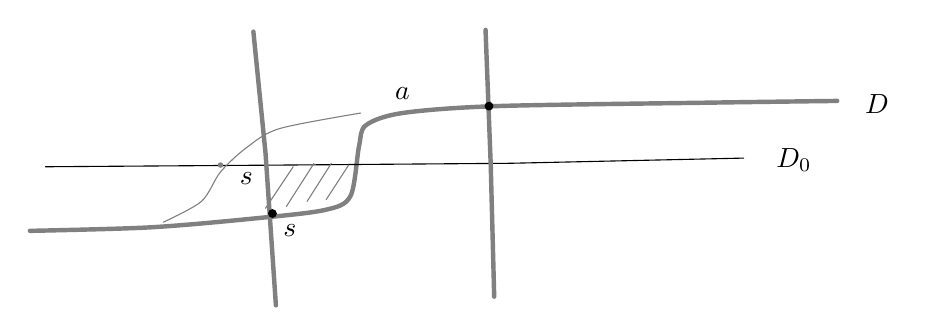
\begin{tikzpicture}[x=0.022cm,y=-0.022cm,line cap=round,line join=round]
\draw[gray,line width=1.6pt] plot[smooth] coordinates {(0,116) (69,114) (128,109) (170,104) (185,96) (190,67) (194,55) (215,48) (269,44) (392,42) (466,41)};
\draw[thin] (9,79)--(149,78)--(277,77)--(412,74);
\draw[gray,line width=1.6pt] (129,1)--(136,71)--(142,159);
\draw[gray,line width=1.6pt] (263,0)--(266,78)--(268,154);
\draw[gray,thin] plot[smooth] coordinates {(77,111) (99,99) (110,82) (125,68) (144,57) (191,48)};
\draw[gray,thin] (136,103)--(152,79);
\draw[gray,thin] (148,102)--(164,77);
\draw[gray,thin] (160,99)--(174,77);
\draw[gray,thin] (171,98)--(184,78);
\fill[black] (140,106) circle [radius=1.6pt];
\fill[black] (265,44) circle [radius=1.6pt];
\fill[gray] (110,78) circle [radius=1pt];
\node at (150,116) {$s$};
\node at (125,86) {$s$};
\node at (215,37) {$a$};
\node at (489,43) {$D$};
\node at (441,75) {$D_0$};
\end{tikzpicture}}

\scanpage{61}
% archive sheet number: 60

\deleted{\deleted{et en choisir} \inserted{d'où une arête privilégiée sur $D$} (celle qui rencontre $D_0$), et je choisis une extrémité $s$, de façon à avoir un repère. Je spécialise $D$ en $D'$ vers le \deleted{pt} \inserted{sommet} $s'$ le plus proche de $s$, je fais un demi-tour par $s$, et je reviens à $D$, --- un nb \deleted{pair} d'opérations, qui change l'orientation de $D$, \uline{et transforme $s$ en $s$} --- donc c'est la symétrie p.r. à $s$. Si on \deleted{fait}}

4.1.

Pour tout \deleted{lacet} chemin \inserted{$c$} combinatoire sur $\Gamma$ --- i.e. chemin formé avec des faces $\unsure{\overline F_D|F_D}$ de $(\mathcal X,K)$, \deleted{\unsure{quel}} allant de la face $F=F_D$ à une $F'=F_{D'}$, on trouve un iso ``de transport parallèle''

\[ \operatorname{Pol}(c):\quad \operatorname{Pol}(F)\longrightarrow\operatorname{Pol}(F'), \]

qui du pt de vue de la géométrie intrinsèque de $(\mathcal X,K,S_K)$ s'interprète par composition successive de ``réflexions'' le long des arêtes de réflexion qui interviennent au cours de $c$.

L'effet de $\operatorname{Pol}(c)$ sur les orientations

\[ \underline{\omega}_x(c):\quad \underline{\omega}(F)\simeq\underline{\omega}(D)\longrightarrow\underline{\omega}(F')\simeq\underline{\omega}(D') \]

est aussi l'effet sur l'orientation des p.r. par transport parallèle --- donc \deleted{est} indépendant de la parité du nb de pas dans le chemin $c$ ! Si on a un lacet \deleted{\unsure{\ell}} $l=c$ i.e. $F=F'$ --- donc

\[ \Pi_1(\mathcal X,F_D)\longrightarrow\underset{\simeq\mathbb D_{2n}}{\operatorname{Aut}(\operatorname{Pol}(D))}\xrightarrow{\substack{\text{effet sur}\\\text{orientation}}}\pm1 \]

on désignera par $\chi_x$ le caractère \unsure{composé}

\[ \chi_x:\Pi_1(\mathcal X,F_D)\longrightarrow\pm1 \]

donc pour un chemin $l$, on aura $\chi_{\unsure{,|x}}(l)=+1$ ou $-1$ suivant que par transport parallèle l'orientation de $D$ aura ou non changé. \deleted{\unsure{On}}

On a deux autres caractères $\chi_s$ et $\chi_a$ (\deleted{\unsure{orient}}ations ``sommets'' et ``arêtes'') en associant à chaque face $F_D$ \deleted{\unsure{les}} deux ensembles à deux éléments

\[ \begin{aligned}
\varepsilon_s(\deleted{\unsure F}F)&=\varepsilon_s(D)=\text{un des \inserted{deux} tronçons inscrits dans }\operatorname{Pol}(D)=\operatorname{Pol}(F),\\
\deleted{\varepsilon_{\unsure{s}}}\varepsilon_{\unsure{a}}(F)&=\varepsilon_a(F)=\text{une des deux \unsure{régions} fermées circonscrites dans }\operatorname{Pol}(D)=\operatorname{Pol}(F)
\end{aligned} \]
